%%%%%%%%%%%%%%%%%%%%%%%%%%%%%%%%%%%%%%%%%%%%%%%%%%%%%%%%%%%%%%%%%%%%%%%%%%%%%%%%
%%%%%%%%%%%%%%%%%%%%%%%%%%%%%%%%%%%%%%%%%%%%%%%%%%%%%%%%%%%%%%%%%%%%%%%%%%%%%%%%
%%                                                                            %%
%% thesistemplate.tex version 4.01 (2023/09/21)                               %%
%% The LaTeX template file to be used with the aaltothesis.sty (version 4.00) %%
%% style file.                                                                %%
%% This package requires pdfx.sty v. 1.5.84 (2017/05/18) or newer.            %%
%%                                                                            %%
%% This is licensed under the terms of the MIT license below.                 %%
%%                                                                            %%
%% Written by Luis R.J. Costa.                                                %%
%% Currently developed at Teacher services, Learning Services of Aalto        %%
%% University by Luis R.J. Costa since May 2019.                              %%
%%                                                                            %%
%% Copyright 2017-2021 aaltothesis.cls by Luis R.J. Costa,                    %%
%% luis.costa@aalto.fi.                                                       %%
%% Copyright 2017-2018 Swedish translations in aaltothesis.cls by Elisabeth   %%
%% Nyberg and Henrik Wallén henrik.wallen@aalto.fi.                           %%
%% Finnish documentation in the template opinnatepohja.tex translated from    %%
%% the English template documentation.                                        %%
%% Copyright 2021 English template thesistemplate.tex by Luis R.J. Costa,     %%
%% Maurice Forget, Henrik Wallén.                                             %%
%% Copyright 2018-2022 Swedish template kandidatarbetsbotten.tex by Henrik    %%
%% Wallen.                                                                    %%
%%                                                                            %%
%% Permission is hereby granted, free of charge, to any person obtaining a    %%
%% copy of this software and associated documentation files (the "Software"), %%
%% to deal in the Software without restriction, including without limitation  %%
%% the rights to use, copy, modify, merge, publish, distribute, sublicense,   %%
%% and/or sell copies of the Software, and to permit persons to whom the      %%
%% Software is furnished to do so, subject to the following conditions:       %%
%% The above copyright notice and this permission notice shall be included in %%
%% all copies or substantial portions of the Software.                        %%
%% THE SOFTWARE IS PROVIDED "AS IS", WITHOUT WARRANTY OF ANY KIND, EXPRESS OR %%
%% IMPLIED, INCLUDING BUT NOT LIMITED TO THE WARRANTIES OF MERCHANTABILITY,   %%
%% FITNESS FOR A PARTICULAR PURPOSE AND NONINFRINGEMENT. IN NO EVENT SHALL    %%
%% THE AUTHORS OR COPYRIGHT HOLDERS BE LIABLE FOR ANY CLAIM, DAMAGES OR OTHER %%
%% LIABILITY, WHETHER IN AN ACTION OF CONTRACT, TORT OR OTHERWISE, ARISING    %%
%% FROM, OUT OF OR IN CONNECTION WITH THE SOFTWARE OR THE USE OR OTHER        %%
%% DEALINGS IN THE SOFTWARE.                                                  %%
%%                                                                            %%
%%                                                                            %%
%%%%%%%%%%%%%%%%%%%%%%%%%%%%%%%%%%%%%%%%%%%%%%%%%%%%%%%%%%%%%%%%%%%%%%%%%%%%%%%%
%%                                                                            %%
%%                                                                            %%
%% An example for writting your thesis using LaTeX                            %%
%% Original version and development work by Luis Costa, changes to the text   %% 
%% in the Finnish template by Perttu Puska.                                   %%
%% Support for Swedish added 15092014                                         %%
%% PDF/A-b support added on 15092017                                          %%
%% PDF/A-2 support added on 24042018                                          %%
%% Layout design and typesettin changed 15072021                              %%
%%                                                                            %%
%% This example consists of the files                                         %%
%%       thesistemplate.tex (version 4.00) (for text in English)              %%
%%       opinnaytepohja.tex (version 4.00) (for text in Finnish)              %%
%%       kandidatarbetsbotten.tex (version 1.10) (for text in Swedish)        %%
%%       aaltothesis.cls                                                      %%
%%       linediagram.pdf (graphics file)                                      %%
%%       curves.pdf      (graphics file)                                      %%
%%       ledspole.jpg    (graphics file)                                      %%
%%                                                                            %%
%%                                                                            %%
%% Typeset in Linux with                                                      %%
%% pdflatex: (recommended method)                                             %%
%%             $ pdflatex thesistemplate                                      %%
%%             $ pdflatex thesistemplate                                      %%
%%                                                                            %%
%%   The result is the file thesistemplate.pdf that is PDF/A compliant, if    %%
%%   you have chosen the proper \documenclass options (see comments below)    %%
%%   and your included graphics files have no problems.                       %%
%%                                                                            %%
%%                                                                            %%
%% Explanatory comments in this example begin with the characters %%, and     %%
%% changes that the user can make with the character %                        %%
%%                                                                            %%
%%%%%%%%%%%%%%%%%%%%%%%%%%%%%%%%%%%%%%%%%%%%%%%%%%%%%%%%%%%%%%%%%%%%%%%%%%%%%%%%
%%%%%%%%%%%%%%%%%%%%%%%%%%%%%%%%%%%%%%%%%%%%%%%%%%%%%%%%%%%%%%%%%%%%%%%%%%%%%%%%
%%
%% WHAT is PDF/A
%%
%% PDF/A is the ISO-standardized version of the pdf. The standard's goal is to
%% ensure that he file is reproducable even after a long time. PDF/A differs
%% from pdf in that it allows only those pdf features that support long-term
%% archiving of a file. For example, PDF/A requires that all used fonts are
%% embedded in the file, whereas a normal pdf can contain only a link to the
%% fonts in the system of the reader of the file. PDF/A also requires, among
%% other things, data on colour definition and the encryption used.
%% Currently three PDF/A standards exist:
%% PDF/A-1: based on PDF 1.4, standard ISO19005-1, published in 2005.
%%          Includes all the requirements essential for long-term archiving.
%% PDF/A-2: based on PDF 1.7, standard ISO19005-2, published in 2011.
%%          In addition to the above, it supports embedding of OpenType fonts,
%%          transparency in the colour definition and digital signatures.
%% PDF/A-3: based on PDF 1.7, standard ISO19005-3, published in 2012.
%%          Differs from the above only in that it allows embedding of files in
%%          any format (e.g., xml, csv, cad, spreadsheet or wordprocessing
%%          formats) into the pdf file.
%% PDF/A-4: based on PDF 2.0, standard ISO19005-4, published in November 2020.
%%
%% PDF/A-1 files are not necessarily PDF/A-2 -compatible and PDF/A-2 are not
%% necessarily PDF/A-1 -compatible.
%% Standards PDF/A-1, PDF/A-2 and PDF/A-3 have two levels:
%% b: (basic) requires that the visual appearance of the document is reliably
%%    reproduceable.
%% a (accessible) in addition to the b-level requirements, specifies how
%%   accessible the pdf file is to assistive software, say, for the physically
%%   impaired.
%% The PDF/A-4 standard does not have additional levels like in the earlier
%% standards.
%% For more details on PDF/A, see, e.g., 
%% https://www.loc.gov/preservation/digital/formats/fdd/fdd000318.shtml or
%% https://www.pdfa.org/resource/iso-19005-pdfa/
%%
%%
%% WHICH PDF/A standard should my thesis conform to?
%%
%% Either to the PDF/A-1b or the PDF/A-2b standard. If all the figures and
%% graphs used in thesis work do not require transparency features, use either
%% PDF/A-1b or PFDF/A-2b. If you have figures with transparency
%% characteristics, use the PDF/A-2b standard. However, drawing applications
%% often use the transparency parameter, setting it to zero, to specify opacity
%% and get the basic 2-D visualisation. As a result, validation of PDF/A-1b
%% will fail. Use PDF/A-2b if PDF/A-1b validation fails.
%% Do not use the PDF/A-3b standard for your thesis.
%% The font to be used are specified in this templatenand they should not be
%% changed. In addition to not adhering to Aalto's visual guidelines, you may
%% have difficulties in producing a PDF/A-compliant PDF.
%%
%%
%% Validate your PDF/A file at https://www.pdf-online.com/osa/validate.aspx
%%
%%
%% WHAT graphics format can I use to produce my PDF/A compliant file?
%%
%% When using pdflatex to compile your work, favour the use of pdf, but you can
%% use the jpg or png format especially for photographs. You will have PDF/A 
%% compliance problems with figures in pdf if the fonts are not embedded in the
%% pdf file.
%% If you choose to use latex to compile your work, the only acceptable file
%% format for your figure is eps. DO NOT use the ps format for your figures.

%% USE one of the following three \documentclass set-ups:
%% * the first when using pdflatex to directly typeset your document in the
%%   chosen pdf/a format for online publishing (centred page layout),
%% * the second for one-sided printing your thesis with the layout (wide left 
%%   margin), or
%% * the third for two-sided printing.
%%
\documentclass[english, 12pt, a4paper, elec, utf8, a-2b, online]{aaltothesis}
%\documentclass[english, 12pt, a4paper, elec, utf8, a-2b, print]{aaltothesis}
%\documentclass[english, 12pt, a4paper, elec, utf8, a-2b, print, twoside]{aaltothesis}

%% Use the following options in the \documentclass macro above:
%% your school: arts, biz, chem, elec, eng, sci
%% the character encoding scheme used by your editor: utf8, latin1
%% thesis language: english, finnish, swedish
%% make an archiveable PDF/A-1b or PDF/A-2b compliant file: a-1b, a-2b
%%                    (with pdflatex, a normal pdf containing metadata is
%%                     produced without the a-*b option)
%% typset for online document or print on paper: online, print
%%        online: typeset in symmetric layout and blue hypertext for online
%%                publishing
%%        print: typeset in a symmetric layout and black hypertext for printing
%%               on paper
%%          two-side printing: twoside (default is one-sided printing)
%%               typeset in a wide margin on the binding side of the page and
%%               black hypertext. Use with print only.
%%

%% Use one of these if you write in Finnish (or use the Finnish template
%% opinnaytepohja.tex)
%\documentclass[finnish, 12pt, a4paper, elec, utf8, a-1b, online]{aaltothesis}
%\documentclass[finnish, 12pt, a4paper, elec, utf8, a-1b, print]{aaltothesis}
%\documentclass[finnish, 12pt, a4paper, elec, utf8, a-1b, print, twoside]{aaltothesis}

%% Use one of these if you write in Swedish (or use the Swedish template
%% kandidatarbetsbotten.tex)
%\documentclass[swedish, 12pt, a4paper, elec, utf8, a-2b, online]{aaltothesis}
%\documentclass[swedish, 12pt, a4paper, elec, utf8, a-2b]{aaltothesis}
%\documentclass[swedish, 12pt, a4paper, elec, dvips, online]{aaltothesis}

%% FOR USERS OF AMS PACKAGES:
%% * newtxmath used in this template loads amsmath, so
%%   you needn't load it. If you want to use options in amsmath, load it here, 
%%   before \setupthesisfonts below to pass the options to amsmath.
%% * If you want to use amsthm, load it here before \setupthesisfonts to avoid
%%   a clash with newtxmath.
%% * If using amsmath with options and you want to use amsthm, load amsthms
%%   after amsmath, as described in the amsthm documentation.
%% * Don't use amsbsym or amsfonts. The symbols [and macros] there are defined in
%%   newtxmath and so clash if used.
%\usepackage[options]{amsmath}
%\usepackage{amsthm}

%% DO NOT MOVE OR REMOVE \setupthesisfonts
\setupthesisfonts

%%
%% Add here the packges you need
%%
\usepackage{graphicx}


%% For tables that span multiple pages; used to split a paraphrasing example in
%% the appendix. If you don't need it, remove it.
\usepackage{longtable}

%% A package for generating Creative Commons copyright terms. If you don't use
%% the CC copyright terms, remove it, since otherwise undesired information may
%% be added to this document's metadata.
\usepackage[type={CC}, modifier={by-nc-sa}, version={4.0}]{doclicense}
%% Find below three examples for typesetting the CC license notice.


%% Edit to conform to your degree programme
%% Capitalise the words in the name of the degree programme: it's a name
\degreeprogram{Electronics and Electrical Engineering}
%%

%% Your major
%%
\major{An appropriate major}
%%

%% Choose one of the three below
%%
%\univdegree{BSc}
\univdegree{MSc}
%\univdegree{Lic}
%%

%% Your name (self explanatory...)
%%
\thesisauthor{Eddie Engineer}
%%

%% Your thesis title and possible subtitle comes here and possibly, again,
%% together with the Finnish or Swedish abstract. Do not hyphenate the title
%% (and subtitle), and avoid writing too long a title. Should LaTeX typeset a
%% long title (and/or subtitle) unsatisfactorily, you might have to force a
%% linebreak using the \\ control characters. In this case...
%% * Remember, the title should not be hyphenated!
%% * A possible 'and' in the title should not be the last word in the line; it
%%   begins the next line.
%% * Specify the title (and/or subtitle) again without the linebreak characters
%%   in the optional argument in box brackets. This is done because the title
%%   is part of the metadata in the pdf/a file, and the metadata cannot contain
%%   linebreaks.
%%
\thesistitle{Title of the thesis}
%\thesistitle[Title of the thesis]{Title of\\ the thesis}
%%
%% Either remove or leave \thesissubtitle{} empty if you don't use it
%%
\thesissubtitle{A possible subtitle}
%\thesissubtitle[Subtitle of the thesis]{Subtitle of\\ the thesis}
%\thesissubtitle{}

%%
\place{Espoo}
%%

%% The date for the bachelor's thesis is the day it is presented
%%
\date{21 September 2023}
%%

%% Thesis supervisor
%% Note the "\" character in the title after the period and before the space
%% and the following character string.
%% This is because the period is not the end of a sentence after which a
%% slightly longer space follows, but what is desired is a regular interword
%% space.
%%
\supervisor{Prof.\ Pirjo Professori}
%%

%% Advisor(s)---two at the most---of the thesis. Check with your supervisor how
%% many official advisors you can have.
%%
\advisor{Dr Alan Advisor}
\advisor{Ms Elsa Expert (MSc)}
%%

%% If you do your thesis work in a company of other institute, give the name of
%% the company or instution here. Otherwise, leave the macro empty, comment it
%% out, or remove it. This will remove this field from the abstract page.
%%
\collaborativepartner{Company or institute name (if relevant)}
%%

%% Aaltologo: syntax:
%% \uselogo{?|!|''}
%% The logo language is set to be the same as the thesis language.
%%
%\uselogo{?}
%\uselogo{!}
\uselogo{''}
%%

%%%%%%%%%%%%%%%%%%               COPYRIGHT TEXT               %%%%%%%%%%%%%%%%%%
%%%%%%%%%%%%%%%%%%%%%%%%%%%%%%%%%%%%%%%%%%%%%%%%%%%%%%%%%%%%%%%%%%%%%%%%%%%%%%%%

%% Copyright of a work is with the creator/author of the work regardless of
%% whether the copyright mark is explicitly in the work or not. You may, if you
%% wish---we encourage you to do so---publish your work under a Creative
%% Commons license (see creativecommons.org), in which case the license text
%% must be visible in the work. Write here the copyright text you want using the
%% macro \copyrighttext, which writes the text into the metadata of the pdf file
%% as well.
%%
%% Syntax:
%% \copyrigthtext{metadata text}{text visible on the page}
%%
%% CHOOSE ONE OF THE COPYRIGHT NOTICE STYLES BELOW.
%% IF USING THE CC TERMS, CHOOSE THE LICENSE YOU WANT TO USE.
%% The different CC licenses are listed at 
%% https://creativecommons.org/about/cclicenses/.
%% If you use the icons from the dolicense.sty package, add the package above
%% (\usepackage{dolicense}).
%% IMPORTANT NOTE!! Manually write the CC text in the \copyrighttext metadata
%% text field.
%%
%% NOTE: In the macros below, the text written in the metadata must have a
%% \noexpand macro before the \copyright special character. When not in pdf/a
%% mode (i.e. a-1b or a-2b are not specified in \documentclass), two \noexpands
%% are required in the metadata text to correctly render the copyright mark in
%% the pdf metadata. In pdf/a mode one \noexpand suffices.
%%
%% EXAMPLE OF PLAIN COPYRIGHT TEXT
%% The macros \copyright and \year below must be separated by the \ character 
%% (space chacter) from the text that follows. The macros in the argument of the
%% \copyrighttext macro automatically insert the year and the author's name.
%% (Note! \ThesisAuthor is an internal macro of the aaltothesis.cls class file).
%%
%\copyrighttext{Copyright \noexpand\textcopyright\ \number\year\ \ThesisAuthor}
%{Copyright \textcopyright{} \number\year{} \ThesisAuthor}
%%
%% Of course, the same text could have simply been written as
%% \copyrighttext{Copyright \noexpand\copyright\ 2018 Eddie Engineer}
%% {Copyright \copyright{} 2022 Eddie Engineer}
%%
%% EXAMPLES OF CC LICENSE: different ways to display the same license
%% 1. A simple Creative Commons license text with a link to the copyright notice:
%\copyrighttext{\noexpand\textcopyright\ \number\year. This work is 
%	licensed under a CC BY-NC-SA 4.0 license.}{\textcopyright{} 
%	\number\year. This work is licensed under a 
%	\href{https://creativecommons.org/licenses/by-nc-nd/4.0/}{CC BY-NC-SA 4.0} 
%	license.}
%
%% To get the URL of the license of your choice, go to 
%% https://creativecommons.org/about/cclicenses/, click on the chosen license
%% you want to use, and copy-and-paste the URL in the macro \href above.
%%
%% 2. A short Creative Commons license text containing the respective CC icons
%% (requires the package dolicense.sty to be added in the preamble as done
%% above) and a link to the corresponding Creative Commons license webpage (see
%% the dolicense package documentation for other license icons):
%\copyrighttext{\noexpand\textcopyright\ \number\year. This work is licensed
%	under a CC BY-NC-SA 4.0 license.}{
%	\parbox{95mm}{\noindent\textcopyright\ \number\year. \doclicenseText} 
%	\hspace{1em}\parbox{35mm}{\doclicenseImage}
%}
%%
%% 3. An expanded Creative Commons license text containing the respective CC
%% icons text and as generated by the dolicense.sty package (the license is set
%% via package options in \usepackage[options]{dolicense} above; see the
%% dolicense package documentation for other license texts and icons):
\copyrighttext{\noexpand\textcopyright\ \number\year. This work is 
	licensed under a Creative Commons "Attribution-NonCommercial-ShareAlike 4.0 
	International" (BY-NC-SA 4.0) license.}{\noindent\textcopyright\ \number
	\year \ \doclicenseThis}
%%%%%%%%%%%%%%%%%%%%%%%%%%%%%%%%%%%%%%%%%%%%%%%%%%%%%%%%%%%%%%%%%%%%%%%%%%%%%%%%


%% The English abstract:
%% All the details (name, title, etc.) on the abstract page appear as specified
%% above.
%% Thesis keywords:
%% Note! The keywords are separated using the \spc macro
%%
\keywords{For keywords choose\spc concepts that are\spc central to your\spc 
thesis}
%%

%% The abstract text. This text in one paragraph is included in the metadata of
%% the pdf file as well as the abstract page. To have paragraphs in your
%% abstract rewrite it in the abstarct environment as described below.
%%
\thesisabstract{%
The abstract is a short description of the essential contents of the thesis
usually in one paragraph: what was studied and how and what were the main
findings. For a Finnish thesis, the abstract should be written in both Finnish
and English; for a Swedish thesis, in Swedish and English. The abstracts for
English theses written by Finnish or Swedish speakers should be written in
English and either in Finnish or in Swedish, depending on the student’s language
of basic education. Students educated in languages other than Finnish or Swedish
write the abstract only in English. Students may include a second or third
abstract in their native language, if they wish. 
The abstract text of this thesis is written on the readable abstract page as
well as into the pdf file's metadata via the thesisabstract macro (see the 
comment in the TeX file). Write here the text that goes into the metadata. The 
metadata cannot contain special characters, linebreak or paragraph break 
characters, so these must not be used here. If your abstract does not contain 
special characters and it does not require paragraphs, you may take advantage of
the abstracttext macro (see the comment in the TeX file below). Otherwise, the 
metadata abstract text must be identical to the text on the abstract page.
}

%% You can prevent LaTeX from writing into the xmpdata file (it contains all the 
%% metadata to be written into the pdf file) by setting the writexmpdata switch
%% to 'false'. This allows you to write the metadata in the correct format
%% directly into the file thesistemplate.xmpdata.
%\setboolean{writexmpdatafile}{false}


%% All that is printed on paper starts here
%%
\begin{document}

%% Create the coverpage
%%
\makecoverpage

%% Typeset the copyright text.
%% If you wish, you may leave out the copyright text from the human-readable
%% page of the pdf file. This may seem like a attractive idea for the printed
%% document especially if "Copyright (c) yyyy Eddie Engineer" is the only text
%% on the page. However, the recommendation is to print this copyright text.
%%
\makecopyrightpage

\clearpage
%% Note that when writing your thesis in English, place the English abstract
%% first followed by the possible Finnish or Swedish abstract.

%% Abstract text
%% All the details (name, title, etc.) on the abstract page appear as specified
%% above. Add your abstarct text with paragraphs here to have paragraphs in the
%% visible abstract page. Nonetheless, write the abstarct text without
%% paragraphs in the macro \thesismacro so that it is added to the metadata as
%% well.
%%
\begin{abstractpage}[english]
  The abstract is a short description of the essential contents of the thesis,
  usually in one paragraph: what was studied and how and what were the main
  findings.

  For a Finnish thesis, the abstract should be written in both Finnish and
  English; for a Swedish thesis, in Swedish and English. The abstracts for
  English theses written by Finnish or Swedish speakers should be written in
  English and either in Finnish or in Swedish, depending on the student’s
  language of basic education. Students educated in languages other than Finnish
  or Swedish write the abstract only in English. Students may include a second
  or third abstract in their native language, if they wish.

  The abstract text of this thesis is written on the readable abstract page as
  well as into the pdf file's metadata via the \verb+\thesisabstract+ macro
  (see comment in this \TeX{} file above). Write here the text that goes onto
  the readable abstract page. You can have special characters, linebreaks, and
  paragraphs here. Otherwise, this abstract text must be identical to the
  metadata abstract text.
  
  If your abstract does not contain special characters and it does not require
  paragraphs, you may take advantage of the \verb+\abstracttext+ macro (see the
  comment in this \TeX{} file below).
\end{abstractpage}

%% The text in the \thesisabstract macro is stored in the macro \abstractext, so
%% you can use the text metadata abstract directly as follows:
%%
%\begin{abstractpage}[english]
%	\abstracttext{}
%\end{abstractpage}

%% Force a new page so that the possible Finnish or Swedish abstract does not
%% begin on the same page
%%
\newpage
%%
%% Abstract in Finnish. Delete if you don't need it. 
%%
%% Respecify those fields that differ from the earlier specification or simply
%% respecify all fields.
\thesistitle{Opinnäyteen otsikko}
\thesissubtitle{Opinnäytteen mahdollinen alaotsikko}
\supervisor{Prof.\ Pirjo Professori}
\advisor{TkT Alan Advisor}
\advisor{DI Elsa Expert}
\degreeprogram{Elektroniikka ja sähkötekniikka}
\major{Sopiva pääaine}
\collaborativepartner{Yhtiön tai laitoksen nimi (tarvittaessa)}
\date{21.9.2023}
%% The keywords need not be separated by \spc now.
\keywords{Vastus, resistanssi, lämpötila}
%% Abstract text
\begin{abstractpage}[finnish]
Tiivistelmä on lyhyt kuvaus työn keskeisestä sisällöstä usein yhtenä kappaleena:
mitä tutkittiin ja miten sekä mitkä olivat tärkeimmät tulokset. Suomenkielisen
opinnäytteen tiivistelmä kirjoitetaan suomeksi ja englanniksi ja ruotsinkielisen
vastaavasti ruotsiksi ja englanniksi. Suomen- tai ruotsinkielisten
opiskelijoiden, joiden opinnäytteen kieli on englanti, tulee kirjoittaa
tiivistelmänsä englanniksi ja koulusivistyskielellään. Muiden kuin
koulusivistyskieleltään suomen- tai ruotsinkielisten tulee kirjoittaa
tiivistelmänsä vain englanniksi. Opiskelija voi halutessaan lisätä
opinnäytteeseensä toisen tai kolmannen tiivistelmän omalla äidinkielellään.
Tämän opinnäytteen tiivistelmäteksti kirjoitetaan opinnäytteen luettavan osan
lomakkeen lisäksi myös pdf-tiedoston metadataan. Kirjoita tähän metadataan
kirjoitettavaa teksti. Metadatatekstissa ei saa olla erikoismerkkejä,
rivinvaiho- tai kappaleenjakomerkkiä, joten näitä merkkeja ei saa käyttää tässä.
Jos tiivistelmäsi ei sisällä erikoimerkkejä eikä kaipaa kappaleenjakoa, voit
hyödynttää makroa abstracttext luodessasi lomakkeen tiivistelmää (katso
kommentti tässä TeX-tiedostossa alla). Metadatatiivistelmatekstin on muuten 
oltava sama kuin lomakkeessa oleva teksti.

\end{abstractpage}

%% Force new page so that the Swedish abstract starts from a new page
\newpage

%% Swedish abstract. Delete it if you don't need it. 
%% 
%% Respecify those fields that differ from the earlier specification or simply
%% respecify all fields.
\thesistitle{Arbetets titel}
\supervisor{Prof.\ Pirjo Professori}
\advisor{TkD Alan Advisor} %
\advisor{DI Elsa Expert}
\degreeprogram{Electronik och electroteknik}
\collaborativepartner{Company or institute name in Swedish (if relevant)}
%\date{21.9.2023}
%% Abstract keywords
\keywords{Nyckelord p\aa{} svenska, temperatur}
%% Abstract text
\begin{abstractpage}[swedish]
Sammandraget är en kort beskrivning av arbetets centrala innehåll: vad 
undersöktes, hur undersöktes det och vilka var de viktigaste resultaten?

I lärdomsprov som skrivs på svenska skrivs sammandraget på svenska och engelska, 
på motsvarande sätt skrivs sammandraget på finska och engelska i lärdomsprov på 
finska. Finsk- eller svenskspråkiga studerande som skriver sitt lärdomsprov på 
engelska ska skriva sammandraget på engelska och på sitt skolutbildningsspråk. 
Studerande vars skolutbildningsspråk inte är svenska eller finska skriver 
sammandraget endast på engelska. Den studerande kan om hen så önskar lägga till 
ett andra eller tredje sammandrag på sitt eget modersmål. Sammandraget fungerar 
då ofta som mognadsprov och bör i så fall vara minst 300 ord långt. Information 
om mognadsprov på svenska finns på MyCourses:\\
\url{https://mycourses.aalto.fi/course/view.php?id=26872}.
\end{abstractpage}


\dothesispagenumbering{}

%% Preface
%%
%% This section is optional. Remove it if you do not want a preface.
\mysection{Preface}
%\mysection{Esipuhe}
I want to thank Professor Pirjo Professor and my instructors Dr Alan Advisor and
Ms Elsa Expert for their guidance.

I also want to thank my partner for keeping me sane and alive.

\vspace{5cm}
Otaniemi, 9 February 2023\\

\vspace{5mm}
{\hfill Eddie E.\ Engineer \hspace{1cm}}

%% Force a new page after the preface
%%
\newpage


%% Table of contents. 
%%
\thesistableofcontents


%% Symbols and abbreviations
\mysection{Symbols and abbreviations}

\subsection*{Symbols}

\begin{tabular}{ll}
$\mathbf{B}$  & magnetic flux density  \\
$c$              & speed of light in vacuum $\approx 3\times10^8$ [m/s]\\
$\omega_{\mathrm{D}}$    & Debye frequency \\
$\omega_{\mathrm{latt}}$ & average phonon frequency of lattice \\
$\uparrow$       & electron spin direction up\\
$\downarrow$     & electron spin direction down
\end{tabular}

\subsection*{Operators}

\begin{tabular}{ll}
$\nabla \times \mathbf{A}$              & curl of vectorin $\mathbf{A}$\\
$\displaystyle\frac{\mbox{d}}{\mbox{d} t}$ & derivative with respect to 
variable $t$\\[3mm]
$\displaystyle\frac{\partial}{\partial t}$  & partial derivative with respect 
to variable $t$ \\[3mm]
$\sum_i $                       & sum over index $i$\\
$\mathbf{A} \cdot \mathbf{B}$    & dot product of vectors $\mathbf{A}$ and 
$\mathbf{B}$
\end{tabular}

\subsection*{Abbreviations}

\begin{tabular}{ll}
AC         & alternating current \\
APLAC      & an object-oriented analog circuit simulator and design tool \\
           & (originally Analysis Program for Linear Active Circuits) \\
BCS        & Bardeen-Cooper-Schrieffer \\ %% dash between the names
DC         & direct current \\
TEM        & transverse eletromagnetic
\end{tabular}


%% \clearpage is similar to \newpage, but it also flushes the floats (figures
%% and tables).
%%
\cleardoublepage

%% Text body begins. Note that since the text body is mostly in Finnish the
%% majority of comments are also in Finnish after this point. There is no point
%% in explaining Finnish-language specific thesis conventions in English.
%% This text will be translated to English soon.
%%
\section{Introduction}
\label{sec:intro}

%% Leave page number of the first page empty
%% 
\thispagestyle{empty}

This is the template file for writing your bachelor’s, master’s or licentiate 
thesis. The template contains parts and text to accommodate the different degree 
levels, bachelor’s and master’s, and so it may contain parts that may not be 
relevant to your thesis. If so, simply delete those parts in the thesis that you
do not need. This applies particularly to the abstract pages, the list of
symbols, the list of abbreviations, and appendices. You may also want to adjust
the template section titles to better suit your work.

The text and comments in this template advise you how to use the template, give 
general pointers on how to write your thesis (you must still refer to writing
guides and converse with your advisor and/or supervisor in this regard), and
provide the technical specifications for the layout and style of the template.

\subsection{Typical content in the introduction}

In principle, the introduction is like the abstract, only broader in scope, and
more detailed. The introduction generally describes the following:

%% An example of an unordered (itemised) list. Instead on the default bullet
%% point, an endash (-- in LaTeX code) is used as the item label.
\begin{itemize}
	\item[--] a description of the background of the field of study, what
	similar work others have already done, as well as an overview of the study,
	\item[--] the goals of the study,
	\item[--] the primary research question and the sub-problems in the line
	of inquiry, and
	\item[--] the scope and constraints of the study along with the main
	concepts involved.
\end{itemize}

Although the introduction is a general description of the study, be concise and 
avoid writing a lengthy introduction. A concise introduction need not have any 
subsections.

%% In a thesis, every section/chapter starts a new page, hence the \clearpage
\clearpage

\section{Literature review}
\subsection{Structure of the thesis}

The thesis comprises the front matter, the main matter and possible appendices.
The front matter in the required order is:

%% An example of an unordered (itemised) list with the default bullet point
%% label.
\begin{itemize}
	\item a cover page,
	\item a page containing copyright information,
	\item the abstract page(s),
	\item an optional preface, and
	\item a table of contents.
\end{itemize}

If the thesis contains mathematical equations, give the list of symbols used to 
represent various quantities along with the mathematical operators used.
The list must contain all the abbreviations used as well. Note that lists of
figures and tables are not required.

The main matter, i.e. the actual thesis, begins after the list of symbols and 
abbreviations. Its structure follows the standard structure used in scientific 
writing. A typical division of the content is
%% An example of an ordered (numbered) list with the default numbering.
\begin{enumerate}
	\item \label{list:intro} Introduction (research objectives and questions)
	\item Literature review (research made earlier in this area)
	\item Research material and methods
	\item Results / Findings
	\item Discussion
	\item \label{list:summary} Summary / Conclusions
	\item References
\end{enumerate}
The parts \ref{list:intro}--\ref{list:summary} in the list above are the text  
of your thesis. Often the discussion and summary (or conclusions) are combined 
in one chapter. The wording of the titles suggested above may differ. As a 
matter of fact, the titles above refer more to the type of content rather than 
being title suggestions. For example, the literature review of a thesis on 
electromagnetics could be under the title ‘Electromagnetic theory and FDTD’. 
The background to the methodology used---FDTD here---could also be in this 
chapter. Note that the chapters and sections within the main matter are 
numbered, and that they appear in the table of contents. The references, or the 
bibliography, is also shown in the table of contents, but without a number 
labelling it.

The appendix or appendices, when necessary, are presented in the last part of
the thesis. They contain things like questionnaires used in the study, 
[selected parts of] data, derivations of mathematical results, a more detailed 
exposition of some aspect in the thesis, or code listings. Number them in the 
table of contents as follows:
%% An example of an ordered list with the capital-letter numbering. The letter
%% nubering is limited to this list only.
\begin{enumerate}
\renewcommand{\labelenumi}{\Alph{enumi}.}
	\item The first appendix
	\item The second appendix
\end{enumerate}

Refer to a suitable guide on writing a thesis for a comprehensive description;
there are plenty of them around. The instructions here are not exhaustive, and
they concentrate more on how to use this template.

A bachelor’s thesis is ideally about 20 pages long, excluding the appendices, 
whereas a master’s thesis is about 60 pages long, again, not counting the pages
in the appendices. The numbers pertaining to the length of your thesis given
here are mere rules of thumb. Consult your school’s thesis guidelines and your 
thesis advisor and/or supervisor for the appropriate length in your case.


\subsection{Page numbering}
Number the pages using Arabic numerals, placed in the centre of the page footer.
The numbering begins from the cover page and runs continuously to the end of the 
thesis. Enter the total number of pages in the thesis---front matter, main
matter and appendices, if present---in the appropriate field on the abstract
page. Enter also the number of pages in the appendices, if present, in the same 
field on the abstract page as follows: total number of thesis pages / number of 
pages in the appendices.

Do not print the page numbers on the cover and the copyright pages; number all
the other pages. Thus, the first page with a page number printed on it---the
first abstract page---is ‘3’. The page numbering of appendices continues from
that on the previous page.


\subsection{Structuring the text in the main matter}
\subsubsection{Sections}

You can structure your text by dividing it into sections with a suitable title. 
Well-devised sectioning clarifies your text, but beware of overusing them, since 
that will fragment and confuse your text. Do not use more than three levels of 
hierarchy in your sections. Notice that the section titles, just as the figure
and table labels, are in a Helvetica clone, a sans serif, or grotesque, font. 
The main matter text is typeset in a Times clone, a serif font.

The sectioning macros available in \LaTeX{} are 
%% \section{title} 
%% \subsection{subtitle}
%% \subsubsection{subsubtitle}
\begin{itemize}
	\setlength{\itemsep}{0pt}
	\item[] \verb+\section{title}+,
	\item[] \verb+\subsection{subtitle}+, and
	\item[] \verb+\subsubsection{subsubtitle}+.
\end{itemize}

The formatting specifications are in appendix~\ref{app:layout}. The fonts 
specified there are for Word documents, as specified by Aalto's visual 
guidelines. No corresponding fonts are officially specified for \LaTeX{}. Hence,
similar corresponding fonts provided by the \verb+newtxtext+ package are used in
this template. Math fonts are those from \verb+newtxmath+. The most important 
factor that influenced this choice of fonts was that the package outputs 
PDF/A-1b compliant pdf using \texttt{pdflatex}.

At least in technical texts, refraining from using the articles ‘a’ and ‘the’ as
the first word in the title is common practice. Appendices are enumerated using 
capital letters. Begin every section on a new page. Begin a subsection on a new 
page only if the previous page is full. Similarly, begin every appendix on a new
page.

\subsubsection{Paragraphs}

The paragraph that follows the section title is not indented, the paragraphs 
that follow are. Often, the body text is typeset as raggedright to avoid 
unnecessarily large white spaces between words. On the other hand, in many 
technical fields, the text is justified on both sides, but in such cases, 
hyphenation is used to maintain reasonable separation between words. This 
template uses justified text with automatic hyphenation. Write paragraphs so 
that they span more than three lines. Rethink your text, if you end up having  
one-line paragraphs; avoid them in your thesis---including the appendices. In 
addition, you may need to reconstruct your text if your paragraphs are too long.
Avoid emphasising text using italics. Italicised text makes reading for dyslexic
readers even more difficult.

When a number has a unit associated with it, ensure two things: the space 
between the number and the unit is smaller than the regular space (for example, 
1\,Hz) and the number and unit are not split over lines. You can simply use 
\verb+\,+ between the number and the unit without spaces between them to stop 
them from being split (\verb+1\,Hz+) or use the package \verb+siunitx+.


\subsubsection{Equations}

Equations are numbered using Arabic numerals, typically enclosed in parentheses,
but not always. This template encloses equation numbers in parentheses. An 
example equation is
\begin{equation}
	f(x) = a_0 + \sum_{n=1}^{\infty} \left( a_n \cos\frac{n\pi x}{L} + 
	b_n \sin\frac{n\pi x}{L} \right).
\end{equation}
Closely related equations like equations in a system of equations may be numbered 
as follows:
\begin{subequations}\label{eq:ohm}
  \begin{alignat}{1}
	V_\text{s} &= R_\text{s} i_\text{s} + R(i_\text{s} + i_\text{b})
	 \label{eq:ohm1}\\
	V_\text{b} &= R_\text{b} i_\text{b} + R(i_\text{b} + i_\text{s}).
	 \label{eq:ohm2}
  \end{alignat}
\end{subequations}
All equations need not be numbered. Remember punctuation after the equation; an
equation is an integral part of your sentence and may need to be followed by 
punctuation marks. Many scientific journals do not use them after equations;
then again, many do. Punctuate the equations in your thesis. Numbering of
equations in appendices consists of the appendix numbering alphabet followed by
the equation number, which starts from one in each appendix. For example, the
first equation in appendix A would be equation~(A1) and the first two 
equations~(A1)--(A2).

\subsubsection{Figures and tables}

Theses generally contain figures and tables, which have captions describing 
them. For figures, the convention is to place the caption after (below) the 
figure, as shown in figure~\ref{fig:coil} and figure~\ref{fig:graph}. Tables, on
the other hand, have the caption above (before), as evident from 
table~\ref{tab:animals}. The label and number are typeset in the sans serif bold
12-pt typeface and the caption in the serif 12-pt normal typeface (see 
appendix~\ref{app:layout}).

%% Example of a figure
%% The environent's optional arguments h (here), t (top), b (bottom) and p
%% (page) try to force LaTeX to place the figure as directed as opposed to being
%% place there where LaTeX deems appropriate. 'p' places the figure on the next
%% page by itself. The order of the arguments determines the preference that is
%% desired. These arguments apply to the table environment as well.
\begin{figure}[tb]
  \centering
  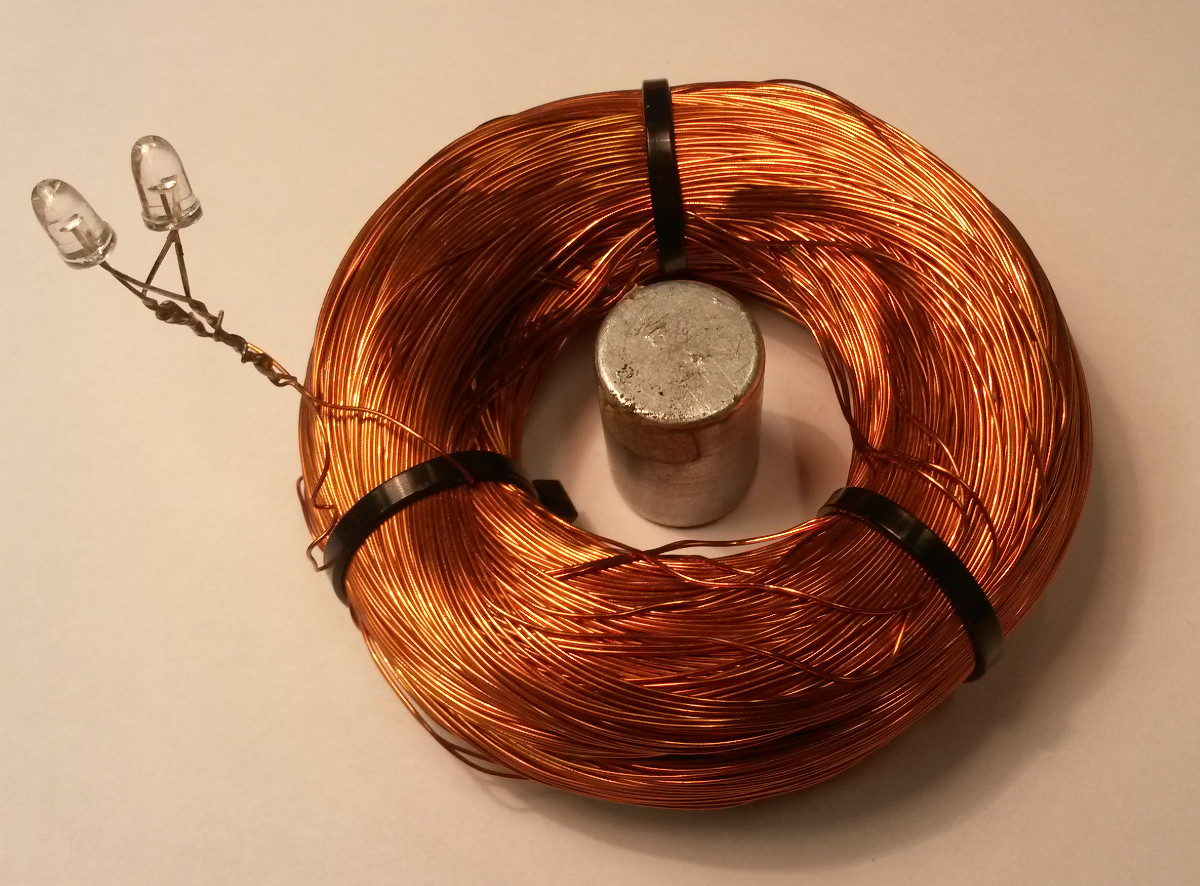
\includegraphics[height=5cm]{./ledspole.jpg}
  \caption{A coil terminated in two LEDs with a magnet placed at its centre.}
  \label{fig:coil}
\end{figure}

\begin{figure}[tb]
  \centering
  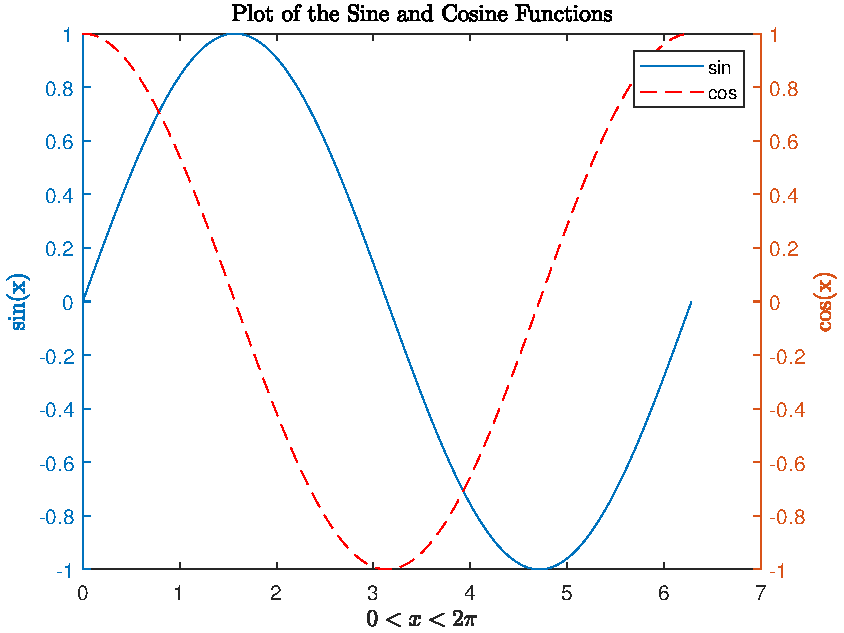
\includegraphics[height=5cm]{curves.pdf}
  \caption{Example of a MATLAB graph.}
  \label{fig:graph}
\end{figure}

%% Example of a table
\begin{table}[tb]
	\centering
	\caption{An example table. Common animals classified into their classes.}
	\label{tab:animals}
	\sffamily% change the font in the table to sans serif
	\begin{tabular}{ccc}
	  \hline
	  \textbf{Mammals} & \textbf{Birds} & \textbf{Insects}\\ \hline
	  dog & crow & ladybird \\ \hline
	  cat & sparrow & ant \\ \hline
	  rat & tit & cockroach \\ \hline
	\end{tabular}
\end{table}

Avoid placing figures and tables such that they are preceded or followed by just
a line or two, because the reader can have difficulties in finding the line(s) 
of text and might even accidentally miss the text completely. Consider, for 
example, a page beginning with one line of text continued from the preceding 
page and that ends the paragraph. This is followed by a figure, then a short 
three-line paragraph, then yet another figure, followed by more text, which is 
positioned such that only two lines of text are on the page and the remainder is
placed on the following page. The layout of this page is fragmented, and as a 
result, the reader might initially miss the top line of text. Consider using one
of the following three layout possibilities: place the figures in the top part 
of the page followed by the text, or place the text in the top followed by the 
figures, or place all the text in the middle with one figure on the top and the 
other at the bottom. Base your choice on considering how easily the reader can 
follow your text (the content of the figures affects this), and whether the page
as a whole looks ordered and pleasing to the eye.

Strive to place the referenced figure or table on the same page as where it is 
referenced. If this is difficult, place it on the following page, but not very 
much further. Using the options \texttt{b} (for bottom), \texttt{t} (for top), 
\texttt{h} (for here) and \texttt{p} (for separate page) judiciously in the 
\texttt{figure} and \texttt{table} environments, \LaTeX{} does a pretty good 
job of placing figures and tables. However, placing figures (and tables) close 
to where they are referred to may be impossible when you have many pictures, so 
use common sense and keep the reader in mind when placing pictures and tables.


\subsection{Referencing parts in the thesis}

Cross-referencing in \LaTeX{} is simple and straightforward: use 
\verb+\label{marker}+ to label the object with a number and then refer to the 
object using \verb+\ref{marker}+. \texttt{marker} should be a unique string of 
characters. To help keep you organised with the various reference labels, be 
systematic when creating them for different objects in the thesis. For example, 
start labels for figures with \texttt{fig:}, for tables with \texttt{tab:}, 
\texttt{sec:} for sections, and \texttt{eq:} for equations, as done in this 
template. So, you could have, say, \verb+\label{sec:ohmslaw}+, 
\verb+\label{eq:ohmslaw}+, \verb+\label{fig:ohmslaw}+, and 
\verb+\label{tab:ohmslaw}+.

Perhaps you will have noticed that when referencing objects in the text, as is 
done for `figure' earlier in the text, the label ‘figure’ in the cross-reference
is not capitalised. Often, you see the capitalised label ‘Figure’. In such 
cases, the label together with the number, for example ‘Figure 2’, is 
considered a proper noun, hence the capitalisation. Although this template uses 
the lowercase form, you can choose how you write cross-referencing labels: 
‘figure’ or ‘Figure’---you will do well to consult your advisor and supervisor 
about this; they may have strong opinions on the matter. However you decide to 
write cross-referencing labels---figure, table, section or equation---be 
consistent.

Do not abbreviate any of the labels, for example ‘figure’ to ‘fig.’ or ‘Fig.’. 
Journals do this because the amount of available space for an article is 
limited; space is not an issue in your thesis. You can refer to more than one 
figure, for example, by saying figures~\ref{fig:coil} and \ref{fig:graph}. Use 
endash `\verb+--+' to specify a range: sections~\ref{sec:intro}--\ref{sec:summary}.

To reference a section, place the section label directly after the sectioning 
command of the section to be referenced. For example:
%% The verbatim environment typesets text within it as-is. Commands are not
%% interpreted and executed within the environment.
\begin{verbatim}
	\subsection{Ohm's law}
	\label{sec:ohmslaw}
	...
	...as discussed in section~\ref{sec:ohmslaw}, the resistance...
\end{verbatim}
The tilde placed between `section' and `\verb+\ref{sec:ohmslaw}+' not only puts 
a normal space between the two, but also binds them so that they are not split 
over separate lines if the two occur at the end of a line. Put a tilde between 
all labels and the reference number.

For figures and tables, place the label text after \verb+\caption+. For simple 
equations, the label is placed after \verb+\begin{equation}+. You can reference
individual items such as equation~(\ref{eq:ohm1}) in a grouped equation 
enviroment like \verb+subequations+ or an item in an itemised list like 
item~\ref{list:intro} on page~\pageref{list:intro} or the system of 
equations~(\ref{eq:ohm}) by putting a \verb+\label+ appropriately.

\subsection{Citation}

The list of reference must be carefully made, following one of many different 
styles. Which you choose depends on the field of your thesis. However, citing 
using footnotes is not allowed in your thesis\footnote{Adding comments in 
footnotes is \underline{not} allowed either.}. A short reference list can have 
entries in the order in which they are cited, but if your list is long, arrange 
the entries in alphabetical order. Read appendix~\ref{app:reference} for a 
fairly thorough discussion of how to cite work in academic writing and make a 
bibliography or list of references. Remember that referencing is a very 
important part of your thesis, so be meticulous and thorough.

\subsubsection{Bibliography or list of references}

Find here a list of some of the typical entries in the bibliography and the 
information they must contain. For a more comprehensive list, see 
\cite{aaltolib}. See appendix~\ref{app:reference} for details on how this 
information must be typeset in different reference styles.\\

\noindent
A \underline{book} entry must contain the following:
\begin{itemize}
\setlength{\itemsep}{-3pt}
\item[--]author(s) 
\item[--]title of the book
\item[--]edition, if there are more than one
\item[--]publisher
\item[--]place of publication
\item[--]time of paublication (typically year)
\item[--]name of series, if the book is part of a series
\end{itemize}
References \cite{Kauranen}--\cite{Koblitz} are examples of books in the 
bibliography. Refering to a particular place in a book, for example like this, 
\cite[s.\ 83--124]{Koblitz}, is a good practice. The reader can thus find the 
referred matter easily.\\

\noindent
The following must be found in an \underline{article} entry:
\begin{itemize}
	\setlength{\itemsep}{-3pt}
\item[--]author(s)
\item[--]title of the article
\item[--]name of the journal or magazine where the article is published
\item[--]volume number of the journal or magazine
\item[--]issue number of the journal or magazine
\item[--]year of publication
\item[--]page numbers of the published article
\end{itemize}
References \cite{bcs}--\cite{Deschamps} are examples of articles in a 
bibliography.\\

\noindent
An \underline{edited book} or \underline{compilation} of contributions, 
typically chapters or articles, from several authors having one or more editors 
or a compiled conference proceedings must have the following information:
\begin{itemize}
\setlength{\itemsep}{-3pt}
\item[--]author(s) of the chapter or part
\item[--]title of the chapter or part
\item[--]mention the kind of publication `In book', or for conference 
proceedings with no editor information use `In' before the name of the 
conference proceedings
\item[--]editor(s) of the compilation identified with (Ed.) or (Eds.)
\item[--]name of the compiled book or conference
\item[--]for a conference article, the time and place where the conference was 
held
\item[--]edition, if more than one
\item[--]place of publication
\item[--]publisher (may not exist for conference proceedings)
\item[--]time (year) of publication
\item[--]pages of cited contribution
\item[--]name of series, if the book is part of one
\end{itemize}
References \cite{Sihvola}--\cite{Lindblom} are examples of references to a part 
of a compilation.\\

\noindent
\underline{Theses} must have the following information:
\begin{itemize}
\setlength{\itemsep}{-3pt}
\item[--]author
\item[--]title of the thesis
\item[--]type of thesis (bachelor's, master's doctoral, other)
\item[--]name of university or institution
\item[--]name of the department, faculty or degree programme
\item[--]location/place of the university or institution
\item[--]year of publication
\end{itemize}
References \cite{Miinusmaa}--\cite{Lonnqvist} are examples of theses in a 
bibliography.\\

\noindent
\underline{Standards} must have the following:
\begin{itemize}
\setlength{\itemsep}{-3pt}
\item[--]standard identifier and number
\item[--]name of the standard
\item[--]edition, if not the first
\item[--]place of publication
\item[--]publisher
\item[--]year of publication
\item[--]number of pages
\end{itemize}
Reference \cite{sfs} is an example of how a standard is entered in a 
bibliography.\\

\noindent
An \underline{interview} entry must have the following details:
\begin{itemize}
\setlength{\itemsep}{-3pt}
\item[--]name of the interviewee
\item[--]position or t academic and/or professional title
\item[--]organisation where the interviewee is placed
\item[--]address of the organisation
\item[--]a mention that the entry is an interview along with the date of the 
interview
\end{itemize}
Reference \cite{interview} is an example of an interview entry in a 
bibliography.

Most scientific articles are available online nowadays and many also in printed 
form. Articles from journals, magazines or other publications available 
\underline{only online} must have the following details in the bibliography:
\begin{itemize}
\setlength{\itemsep}{-3pt}
\item[--]author(s)
\item[--]name of the article
\item[--]name of the publication (journal or magazine)
\item[--]type of publication
\item[--]edition or volume
\item[--]volume number and issue details of publication and article
\item[--]year of publication along with details on possible updates: Updated, 
date of update
\item[--]mention `Accessed' and date when accessed
\item[--]mention `Available' and URL or mention `DOI' ja DOI number (DOI=Digital
Object Identifier).
\end{itemize}
References \cite{Ribeiro}--\cite{kone} are examples of how theses available 
online are presented in a reference list. Additionally, references 
\cite{Ribeiro} and \cite{Stieber} available both online as well as in print, so 
the details are presented as for the corresponding entry in print and the 
details of the online version are also given. Reference \cite{kone} is 
available only online, so only those relevant required details are given.
Unfortunately, the details on the edition, publication name and number are 
often unavailable and so cannot be presented in the reference list.\\

\noindent
For a \underline{thesis that is only available online}, give the following 
details:
\begin{itemize}
\setlength{\itemsep}{-3pt}
\item[--]author
\item[--]thesis title
\item[--]type of medium (online, DVD, CD-ROM etc.)
\item[--]type of thesis (bachelor's, master's doctoral, other)
\item[--]name of institution or university
\item[--]name of the department, faculty or degree programme
\item[--]location/place of the university or institution
\item[--]year of publication
\item[--]date of citation
\item[--]availability: mention `Available' and give the URL and/or mention `DOI'
and the DOI number
\end{itemize}
Reference \cite{Adida} is an example of how a thesis available in electronic 
form is entered in a bibliography.\\

\noindent
Reference \cite{webpage} is an example of an online stand-alone article, one not
associated with any journal or magazine. Such an article is considered a work of
its own. The details required of such a \underline{stand-alone webpage} 
are:
\begin{itemize}
\setlength{\itemsep}{-3pt}
\item[--] author(s)
\item[--] title
\item[--] mention `Updated' and date of update
\item[--] mention `Accessed' and date of access
\item[--] mention `Available' and the URL
\end{itemize}
If the article spans more than one page, the reference list must contain the URL
of the page pointing to the entire article, typically its homepage, unless the 
intention is to cite a particular page in the article.


\clearpage

\section{Research material and methods}

This part is the core of your work, where you explain the methodological choices
you made, its limitations, how you pick your research material or subjects, the 
implementation of your study and the methods used. This section determines the 
methodological strengths and weaknesses of your thesis. Any earlier description 
of the method should limit itself to work done earlier by others. Here you tell 
your reader what you have done.

\clearpage

\section{Results}

Present the results of your study here and answer the research questions, asked 
earlier in the thesis (in the introduction, perhaps), this study strives to 
answer. The scientific value of your work is measured by the results you obtain 
along with the arguments you give to back the answers to your research 
questions.

Be critical of the significance of your results. You may critically scrutinise 
the results and your interpretation of the results here, or you may do so later 
in the chapter with the discussion of your work or in the conclusions part.

This part should discuss how reliable the data used in the study are. You may 
discuss the reliability of the conclusions drawn from the study either in this 
chapter or later in the discussions part. You may have the discussion in a 
chapter of its own, separate from the summary or conclusions.


\clearpage

\section{Summary/Conclusions}
\label{sec:summary}

This is where you tie up any loose ends. Tell your reader briefly and clearly 
what you have done, what you have discovered, and the value of your discovery 
in the context of similar work done earlier. Draw clear conclusions regarding 
the research problem, sub-problems or hypotheses. You also discuss future lines 
of study and new questions your study might have posed.

As the author of the thesis, you alone are responsible for ensuring that the 
layout, form and structure of your thesis adheres to the guidelines outlined by 
your school. This template aims to help you meet these requirements.



\clearpage
%% Bibliography/ list of references
%%
\thesisbibliography

\begin{thebibliography}{99}

%% A quick-and-dirty hack to add text between the bibliography section title
%% and the first reference. You don't need this in your thesis, so remove it.
  \item[]
  \hskip-\leftmargin
  \begin{minipage}{\textwidth}
	This is the list of references to the sources cited in 
	appendix~\ref{app:layout}. The list more or less follows the Vancouver 
	style (IEEE). See appendix~\ref{app:reference} for a detailed exposition 
	on cross-referencing and bibliography styles. Follow the description there.
  \end{minipage}
  \bigskip
%% End of hack.

  \bibitem{aaltolib} Citation Guide: Making a bibliography, \textit{Aalto 
  	University Learning Centre}. Online article. Available  
    \url{https://libguides.aalto.fi/c.php?g=410674&p=2797572}
    (accessed on 14.7.2021)

  \bibitem{Bringhurst} Bringhurst, R., \textit{Horizontal Motion. The Elements 
  	of Typographic Style}, Point Roberts, WA: Hartley \& Marks, 1992. p. 26, 
    pp.\ 25--36. Also available online as version 3.0 at  
    \url{https://smallpressblog.files.wordpress.com/2017/11/bringhurstelementsselections1.pdf} (accessed on 7 May 2021).

  \bibitem{Unna} de Buen Unna, J., \textit{Manual de dise\~no editorial}, 4. ed. 
    corrigida y aumentada, Somonte-Cenero, Gij\'on: Ediciones Trea, 2014.

  \bibitem{Dyson} Dyson, M. C., and Kipping, G. J., ``The Effects of Line Length 
    and Method of Movement on Patterns of Reading from Screen,'' 
    \textit{Visible Language,} vol.~2, no.~2, pp. 150--181, 1998.

  \bibitem{Shaik} Shaikh, A. D., ``The Effects of Line Length on Reading Online 
    News,'' \textit{Usability News}, vol.~7, no.~2, July 2005.

  \bibitem{Bailey} Bailey, C., \textit{The Basics of Typography}. [Online].
    \url{https://www.webfx.com/blog/web-design/the-basics-of-typography} 
    (accessed on 14 July 2021).

  \bibitem{Wikilinelength} Wikipedia contributors, ``Line length,'' 
    \textit{Wikipedia: The Free Encyclopedia}, Wikimedia Foundation, Inc., 
    22 July 2004.
    \url{https://en.wikipedia.org/w/index.php?title=Line_length&oldid=997524503}
    (accessed 7 May 2021).

  \bibitem{enwiki:1026690618} Wikipedia contributors, ``Leading,'' 
    \textit{Wikipedia, The Free Encyclopedia}, 2021.
    \url{https://en.wikipedia.org/w/index.php?title=Leading&oldid=1026690618}
    (accessed 14 July 2021).

  \bibitem{aaltovisual} ``Visual elements,'' \textit{Aalto University Brand 
  	Library}. [Online].
	\url{https://www.aalto.fi/en/brand-library#/visual-elements/typography} 
    (accessed 14 July 2021)

\newpage
%% The same hack again
  \bigskip
  \item[]
  \hskip-\leftmargin
  \begin{minipage}{\textwidth}
	The reference list that follows are examples containing the required 
	information about the cited sources, and it more or less abides to the 
	Vancouver style (IEEE). See appendix~\ref{app:reference} for guidelines for 
	making your reference list correctly.
  \end{minipage}
%\medskip
%%

  \bibitem{Kauranen} Kauranen, I., Mustakallio, M. and Palmgren, V., 
    \foreignlanguage{finnish}{\textit{Tutkimusraportin kirjoittamisen opas opinnäytetyön tekijöille}, 
    Espoo, Teknillinen korkeakoulu,} 2006.

  \bibitem{Itkonen} Itkonen, M., \textit{Typografian käsikirja}, 3rd edition, 
	Helsinki, RPS-yhtiöt, 2007.

  \bibitem{Koblitz} Koblitz, N., \textit{A Course in Number Theory and 
  	Cryptography. Graduate Texts in Mathematics 114}, 2nd edition, New York, 
    Springer, 1994.

%% Note the '\' character after the full-stop and the capitalised initial in
%% the author's name. It forces a normal-sized space between the full-stop and
%% the initial. Otherwise a capital letter after a full-stop would imply the
%% start of a new sentence, putting a space a little longer than normal.
  \bibitem{bcs} Bardeen, J., Cooper, L.\ N. ja Schrieffer, J.\ R., ``Theory of 
    Superconductivity,'' \textit{Physical Review,} 1957, vol.~108, no.~5, 
    pp.\ 1175--1204.

  \bibitem{Deschamps} Deschamps, G.\ A., ``Electromagnetics and Differential 
    Forms,'' \textit{Proceedings of the IEEE,} 1981, vol.~69, no.~6, pp.\ 
    676--696.

  \bibitem{Sihvola} Sihvola, A. et al., ``Interpretation of measurements of 
    helix and bihelix superchiral structures,'' in: Jacob, A.\ F. and Reinert, 
    J. (Eds.) \textit{Bianisotropics '98 7th International Conference on Complex
    Media}, Braunschweig, 3.--6.6.1998, Braunscweig, Technische Universität 
   Braunschweig, 1998, pp.\ 317--320.

%% An example of how to force hyphenation in Finnish. Note the use of quotation
%% marks. \foreignlanguage affects quotation marks, since their use differs in
%% different languages. Since this work is in English, the quotaion marks are
%% used as they should be in English and hence are outside the marco.
  \bibitem{Lindblom} Lindblom-Ylänne, S. and Wager, M.,
    ``\foreignlanguage{finnish}{Tieteellisten opinnäytetöiden ohjaaminen},'' in:
    Lindblom-Ylänne, S. and Nevgi, A. (Eds.), \textit{Yliopisto- ja
    korkeakouluopettajan käsikirja}, Helsinki, WSOY, 2004, pp.\ 314--325.
 
  \bibitem{Miinusmaa} Miinusmaa, H., \textit{Neliskulmaisen reiän poraamisesta
	kolmikulmaisella poralla}, Master's thesis, Teknillinen korkeakoulu,
	Department of Mechanical Engineering, Espoo, 1977.
 
  \bibitem{Loh} Loh, N.\ C., \textit{High-Resolution Micromachined 
  	Interferometric Accelerometer}, Master's thesis, Massachusetts Institute of 
    Technology, Cambridge, Massachusetts, 1992.

  \bibitem{Lonnqvist} Lönnqvist, A., \textit{Applications of hologram-based 
  	compact range: antenna radiation pattern, radar cross section, and absorber 
  	reflectivity measurements}, Doctoral thesis, Teknillinen korkeakoulu, 
    Department of Electrical and Telecommunications Engineering, 2006.

  \bibitem{sfs} SFS 5342, \textit{Kirjallisuusviitteiden laatiminen}, 2nd 
    edition, Helsinki, Suomen standardisoimisliitto, 2004. 20~p.

  \bibitem{interview} Palmgren, V., Planning Officer, Teknillinen korkeakoulu, 
    library, Otaniementie 9, 02150 Espoo. Interview, 15.1.2007.

  \bibitem{Ribeiro} Ribeiro, C.\ B., Ollila, E. and Koivunen, V., ``Stochastic 
	Maximum-Likelihood Method for MIMO Propagation Parameter Estimation,'' 
	\textit{IEEE Transactions on Signal Processing}, vol.~55, no.~1, pp. 46--55.
	[Online]. Accessed 19.1.2007. Also available in print.
	DOI: 10.1109/TSP.2006.882057.

  \bibitem{Stieber} Stieber, T., ``GnuPG Hacks,'' \textit{Linux Journal.} Online
	publication, 2006, November, no.~143. Accessed 19.1.2007. Also available in 
	print. Available: \url{http://www.linuxjournal.com/article/8732.}

  \bibitem{kone} Pohjois-Koivisto, T., ``\foreignlanguage{finnish}{Voiko kone 
  	tulevaisuudessa arvata tahtosi?,}'' \textit{Apropos.} Online publication, 
	February, no.~1, 2005. Accessed 19.1.2007. Available:
	\url{http://www.apropos.fi/1-2005/prima.php.}

  \bibitem{Adida} Adida, B., \textit{Advances in Cryptographic Voting Systems}, 
	PhD Thesis, Massachusetts Institute of Technology, Cambridge, Massachusetts,
	2006. Online document. Accessed 19.1.2007. Available: 
	\url{http://crypto.csail.mit.edu/~cis/theses/adida-phd.pdf.}

  \bibitem{webpage} Kilpeläinen, P., 
    \textit{\foreignlanguage{finnish}{WWW-lähteisiin viittaaminen 
    		tutkielmatekstissä}.} Online article. Updated 26.11.2001. 
	Accessed: \url{http://www.cs.uku.fi/~kilpelai/wwwlahteet.html.}

\end{thebibliography}

%% Appendices
%% If you don't have appendices, your thesis ends here. Remove \clearpage,
%% \thesisappendix and the following text below. The last command of this file
%% is \end{document}.
\clearpage

\thesisappendix

\section{Contents of an appendix}
\label{app:contents}

Appendices are not essential in a thesis, and so you must plan the content of 
your thesis as if it does not contain an appendix. The appendix cannot be used 
as a dumping ground for text and ideas from an overgrown thesis.

An appendix is an independent entity, even though it complements the thesis. 
So, the appendix is not, say, just a list or image or table, but contains 
explanatory text as well that indicates the purpose of its content. It can 
contain code listings, like the one below for a simplified list of commands to 
create an appendix.
\begin{verbatim}
	\clearpage
	\appendix
	\addcontentsline{toc}{section}Contents of an appendix}
	\thispagestyle{empty}
	\section*{Contents of an appendix}
	...
	text
\end{verbatim}

Equation numbering in the appendix forms a separate, complete entity. Here are a couple of examples how equations in an appendix are numbered:
\begin{align}
	(x+a)^n &= \sum_{k=0}^n \binom{a}{b} x^n a^{n-k}, \label{appeq:1}\\
	\sin\alpha \pm \sin\beta &= 2\sin\left(\frac{\alpha\pm\beta}{2}\right)
	\sin\left(\frac{\alpha\mp\beta}{2}\right). \label{liitekaava2}
\end{align}

The appendix can contain figures that do not fit in to complement the text in 
the thesis. The numbering of figures is like that of equations: see figure~\ref{appfig:refraction}.

%% Example of a figure in the appendix. Note how b places the figure at the
%% bottom of the page.
\begin{figure}[b]
	\centering
		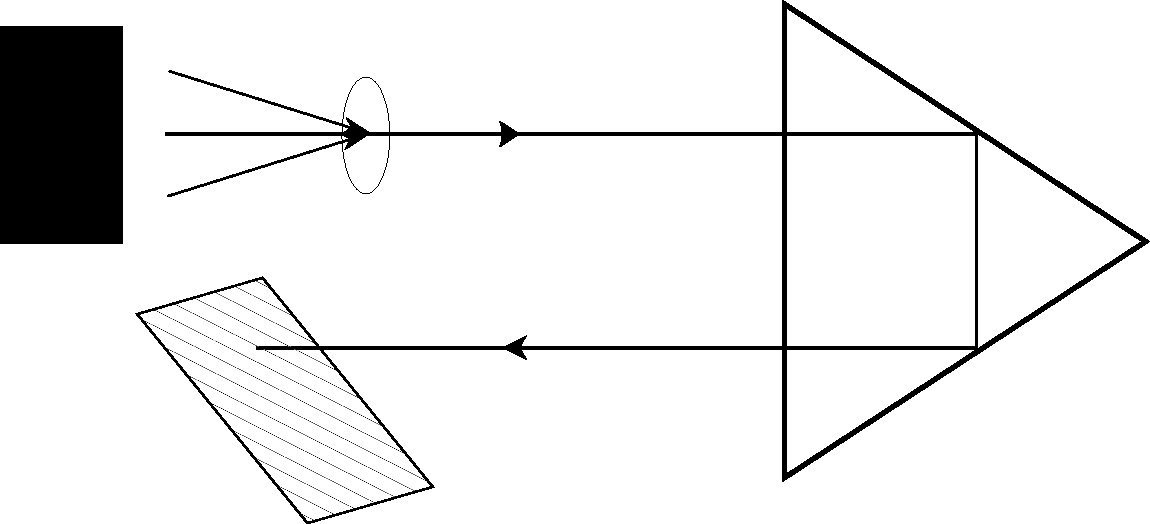
\includegraphics[height=31mm]{./linediagram.pdf}
	\caption{Figure and caption to show the numbering in the appendix.}
	\label{appfig:refraction}
\end{figure}

The numbering of tables is like that for equations and figures, as is evident 
from the caption of table~\ref{apptab:schedule}.

%% Example of a table in the appendix. Note how h places the table in the
%% current position.
\begin{table}[htb]
	\centering
	\caption{Caption for the table.}
	\label{apptab:schedule}
	\sffamily% change the font in the table to sans serif
	\fbox{
		\begin{tabular}{lp{0.5\linewidth}}
			9.00--9.55  & Safety instructions on the use of laboratories\\
			9.55--10.00 & Transfer to the laboratory
		\end{tabular}}
\end{table}


\clearpage
\section{Page layout and typographical design}
\label{app:layout}

\subsection*{Layout choices}

Designing a visually pleasing, balanced and easily readable document requires 
setting several typographic parameters, one of the most important ones being the
line length. If too wide, the reader’s eyes have trouble focusing on the text 
because the line length makes it difficult to gauge when the line begins and 
where it ends; too narrow, and the reader’s eyes have to travel back too often, 
breaking their reading rhythm and often causing them to begin the next line 
before finishing the current one.

Traditional research on the effect of line length on readability of printed text
have found that 45--75 characters per line (cpl) is an acceptable range, with 
66\,cpl being the ideal \cite{Bringhurst, Wikilinelength}. This number includes 
letters, numbers and spaces. The line length in conventional books tends to be 
30 times the type size, but anything between 20 and 40 times is considered 
acceptable. For example, for a 10-pt font, an acceptable line length is 300 
points (30$\times$10), or about 10,58\,cm. The reader’s experience as a reader 
also affects the preferred line length; an experienced reader can handle between
45 and 80\,cpl for a comfortable reading experience, whereas a novice prefers a 
line length of between 34 and 600\,cpl \cite{Unna}.

\begin{figure}[b]
	\centering
	\fbox{\parbox{300pt}{\footnotesize Lorem ipsum dolor sit amet, consectetur 
			adipiscing elit. Pellentesque et urna posuere, aliquam risus et, 
			ullamcorper quam. Pellentesque sed dignissim metus. Etiam turpis 
			dui, suscipit sed libero vel, vulputate imperdiet risus. Sed rutrum
			magna nec neque ornare, at imperdiet sapien porttitor. Sed
			fringilla, enim nec sollicitudin laoreet, arcu leo convallis nisl, 
			eget rhoncus ligula libero malesuada justo.}}
	\caption{Text typeset in a 300-pt-wide box using a font size of 10\,pt. The 
		resulting average number of characters per line is about 60. The text is
		framed to make the box size evident.}
\end{figure}

Reading text from a screen poses challenges absent in paper: glare, flicker and 
scrolling. Research seems to indicate that longer lines are better for scanning 
through the text whereas shorter lines are preferred for accurate reading. One 
study says that reading speed at a certain level of comprehension seems to be 
better for longer lines (100\,cpl) than for shorter lines (25\,cpl) 
\cite{Dyson}. Another study \cite{Shaik} indicates that subjective preferences 
for longer or shorter line lengths appear to be contradictory. About 60\% of 
the test subjects preferred the presented shortest (35\,cpl) or longest 
(95\,cpl) lines, and at the same time all of them disliked either the 
shortest or the longest lines. (See also \cite{Wikilinelength}.)

Another important typographical parameter is line leading or leading, which 
refers to the distance between adjacent lines of text. Double spacing is a 
practice from the era of typewriters particularly in academia to allow making 
handwritten comments in documents. Typewriters had a limited number of options 
for leading, and double spacing was chosen as a norm. Too much leading can cause
continuity problems, since the reader’s eyes must travel a greater distance 
between lines of text. The amount of leading is a compromise between ease of 
reading, desired efficiency in the use of vertical space, weight and type (serif
or sans serif) of the typeface used, and visual aesthetics. Naturally, whether a
document is printed or published online affects the leading, but even the 
language of the text must be considered when deciding on the required leading. 
(See also \cite{enwiki:1026690618}.)

\subsection*{Aalto University’s visual guideline for writing documents}

Of Aalto University’s visual guidelines \cite{aaltovisual}, the one that applies
to document writing is related to the use of fonts. This guideline specifies 
that the body of the text be in the serif font Sentinel and the sec-tion titles 
in boldface of the sans serif font Nimbus Sans. These fonts should be available 
on all Aalto computers. However, being a commercial product, Sentinel can be 
replaced with Georgia and Nimbus Sans with Arial, both of which come installed 
in all Windows machines. Thus, Georgia and Arial are the fonts used in the Word 
template. The font choices for this \LaTeX{} template are a Times and Helvetica 
clone from the \verb+newtxtext+ package since it provides support for math fonts
and its output is a PDF/A compliant pdf.

\subsection*{Layout and typographical specifications}
\subsubsection*{Page layout in the thesis}

The thesis is typeset on A4-sized paper. The text width is set to an average of 
about 75\,cpl as a compromise between having to read the thesis on a computer 
screen and on paper, as discussed above. For the font size of 12\,pt to be used 
in the body text, the text width works out to 14,2\,cm. For the online version 
of the document, the text column is centred, implying that the left and right 
margins are both 3,4\,cm. If you want to print the document and bind it, the 
binding margin must be 4,8\,cm. The text height is set to 23\,cm by setting the 
top margin to 3,7\,cm and the bottom margin to 3\,cm. The layout dimensions are 
summarised in table~\ref{tab:layout}.

\begin{table}[htb]
	\centering
	\caption{Page layout dimensions.}
	\label{tab:layout}
	\sffamily% change the font in the table to sans serif
	\begin{tabular}{ll}
		\hline
		Paper size & A4\\\hline
		Text width & 14,2\,cm \\\hline
		Top margin & 3,7\,cm \\\hline
		Bottom margin & 3,0\,cm \\\hline
		\textbf{Online document} & \\\hline
		Left margin & 3,4\,cm \\\hline
		Right margin & 3,4\,cm \\\hline
		\textbf{Printed document} & \textbf{(for binding)} \\\hline
		Left margin & 4,8\,cm \\\hline
		Right margin & 2,0\,cm \\\hline
	\end{tabular}
\end{table}


\subsubsection*{Sectioning and text body}

The font for the body text is a 12-pt serif Times clone and a Helvetica bold 
clone for the section titles. Use at most three levels of hierarchy in your 
text: section, subsection and subsubsection. The lower section numbering must 
use the section number of the higher section. For example, section number 2.1.3 
refers to section 2, subsection 1 and subsubsection 3.

\clearpage
\section{Reference and in-text citation guidelines}
\label{app:reference}

With regard to standard practice across academic disciplines, it is important to
use an in-text citation to indicate when your work borrows or refers to words or
ideas from a specific source. A full reference of this source should be included
in your ‘References’ / ‘Bibliography’ / ‘Works Cited’ section as well.

There are two major referencing styles: the Harvard style and the Vancouver 
style. The former was first introduced in a journal article by Professor of 
Zoology Edward Marks in 1881 during his tenure at Harvard University (Chernin, 
1988, 1062). It has since become an umbrella term to refer to styles which 
utilise author-date (e.g., APA style) or author-page (e.g., MLA style) within 
parentheses (). It still remains in use to some degree in the natural sciences 
(e.g., American Chemical Society, 2006) and has become the predominant style 
within the social sciences (e.g., American Psychological Association, 2010), and
the arts and humanities (e.g., Modern Languages Association, 2016; University of
Chicago Press, 2017). In contrast, the latter Vancouver style has become a very 
common style within the fields of engineering, technology and science. The name 
is derived from the inaugural meeting in Vancouver, Canada in 1978 of a 
committee later referred to as the International Committee of Medical Journal 
Editors (ICMJE) (BMA, 2012). The style is typified by its use of numbers for 
in-text citations; as such, it is also known as the author-number system. One of
the most common versions of the Vancouver Style is the IEEE Reference Guide \\
(IEEE 2018). The numbers used for in-text citations correspond to a numbered 
reference list at the end of the text. Typically, the numbers refer to the order
in which the referenced authors first appear in the text. Thereafter, they 
continue to be referred to by this number. A lesser utilised variation of this 
style can feature the numbers corresponding to an alphabetical list of authors.

There is a third system of notes and bibliography. This is one of the two styles
in the Chicago Manual of Style; the other is an author-date style. Notes and 
bibliography is mostly used by the fields of literature and history. It is 
occasionally utilised in the field of arts, but it is considerably less common 
than the Harvard style. Among the 97 English doctoral dissertations available 
online in AaltoDoc as of 5 March 2020, only 14 utilised this method. As it is 
relatively rare within Aalto University, it is recommended to visit the Chicago 
Manual of Style online for the reference style guide for it.

The two key considerations in adopting a particular style are that you agree 
with your supervisor on the particular style at the start of your thesis writing
process and that you remain consistent in the use of the style throughout your 
thesis. Your supervisor can provide recommendations for you on the common style 
guides generally used in your field.

Below, you will find general guidelines to these two major styles with reference
to the specific style guides in use. Corresponding examples are provided in the 
boxes below. Please note that the use of boxes here is only to visually separate
the examples for clarity’s sake and that boxes should not be used when quoting 
or paraphrasing in your own thesis.


\subsection*{Direct quotes}

If you are using the exact wording from a source, you should place this in 
double quotation marks (“ ”) followed by the author, date, and page number in 
parentheses (if using the Harvard style) or a number in square brackets [if 
using the Vancouver style]. The citation should be on the same line and inside 
the punctuation. This citation should correspond to a full reference in the 
References / Bibliography / Works Cited section of your thesis. The punctuation 
used between the author, date, and page number may vary depending on which style
guide you are using (compare, for example, The Chicago Manual of Style 
(University of Chicago Press, 2017), The Publication Manual of the American 
Psychological Association (APA, 2018), The MLA Handbook (MLA, 2016) and The New 
Oxford Style Manual (OUP, 2016)). However, it should be noted that the frequency
of direct quote usage varies significantly between academic fields. While it is 
a fairly common practice to utilise quotes within art, design, architecture and 
business, it is rare in the science and engineering fields. Therefore, it is 
recommended that you ask your supervisor or check well-known journals in your 
field to gauge the frequency of quoting preferred by experts in your field.


\subsubsection*{Quoting in Harvard style}

\newcounter{example}[section]
\refstepcounter{example}
\textsf{\textbf{Example~\theexample:}} Quote, information-prominent, American 
Sociological Association (2019) style

\vspace{1ex}
\noindent
\fbox{\parbox{\textwidth-2\fboxsep}{\textsf{
	Attending to these breakdowns not only result in an on-going re-constitution
	of relations between people and things but are also hotbeds for unleashing 
	everyday “creativity, invention, imagination, and artfulness” (Jackson, 
	2014: 226).
	}}}

\vspace{1ex}
\noindent
\textit{Source:} Durrani, M. 2018. Designers by any other name: exploring the 
sociomaterial practices of vernacular garment menders. \textit{Design Research 
Society International Conference: Catalyst. DRS International Conference 
Series.} 4: 1731-1746. ISBN 978-1-912294-19-0 (electronic). 
DOI: 10.21606/dma.2018.495. \copyright{} 2018 Design Research Society. This work
is licensed under a Creative Commons Attribution-NonCommercial-ShareAlike 4.0 
International License. \url{https://creativecommons.org/licenses/by-nc-sa/4.0/.}

\vspace{1em}
\noindent
\refstepcounter{example}
\textsf{\textbf{Example~\theexample:}} Quote, author-prominent, American 
Psychological Association (2010) style

\vspace{1ex}
\noindent
\fbox{\parbox{\textwidth-2\fboxsep}{\textsf{
	Philosopher Mark Johnson (2007) argued that meanings emerge from “deeper 
	explorations into the qualities, feelings, emotions, and bodily processes” 
	(p. x).
}}}

\vspace{1ex}
\noindent
\textit{Source:} Aktaş, B. \& Mäkelä, M. (2019). Negotiation between the maker 
and material: Observations on material interactions in felting studio. 
\textit{International Journal of Design}, 13(2): 55--67. \copyright{} 
\textit{2019 Aktaş \& Mäkelä. Copyright for this article is retained by the 
	authors, with first publication rights granted to the International Journal 
	of Design. All journal content, except where otherwise noted, is licensed 
	under a Creative Commons Attribution-NonCommercial-NoDerivs 2.5 License.}


\subsubsection*{Block quoting}

Block quotes are used for longer quotes. Note the line indentation on each line 
of the block quote below, starting from “There was \ldots”, and the absence of 
quotation marks. Each style guide recommends its own minimum text length before 
using block quoting. [Compare: AMA - four lines of text or more; APA - 40 words 
or more; or Chicago - 100 words or more.]

\vspace{1em}
\noindent
\refstepcounter{example}
\textsf{\textbf{Example~\theexample:}} Block quote, Harvard style, as 
recommended by journal

\vspace{1ex}
{\centering
\fbox{\parbox{\textwidth-2\fboxsep}{\textsf{
	When the Center for Bits and Atoms won the National Science Foundation Grant
	in 2003, MIT engineers began to look for local communities around the world 
	they could help via digital fabrication: “Instead of bringing information 
	technology to the masses, the fab labs bring information technology 
	development to the masses,” explained Gershenfeld, in the official press 
	release (NSF 2004). Karlsen had a more colourful version:\\[1em]
	\mbox{}\hfill\parbox{125mm}{There was an innovation competition launched by 
		MIT globally to develop local projects. MIT sent some of its best 
		teachers to Norway to find a suitable cooperation project. They found us
		through Telenor, who told them: ‘There is this crazy guy lost in the 
		fjord who devised sensors for his animals.’ We enjoyed a great year of 
		cooperation with MIT in 2001 and we were invited to Boston to present 
		and develop this project.}
}}}
}

\vspace{1ex}
\noindent
\textit{Source:} Kohtala, C \& Bosqu\'e, C. (2014). The Story of MIT-Fablab 
Norway: Community Embedding of Peer Production. Journal of Peer Production, 
5 (8): 1--8. ISSN 2213-5316 (electronic). \copyright{} 2014 public domain.  \url{http://peerproduction.net/issues/issue-5-shared-machine-shops/peer-reviewed-articles/the-story-of-mit-fablab-norway-community-embedding-of-peer-production/}


\subsection*{Paraphrasing}

Paraphrasing is a more prevalent citation practice in many academic fields. In 
engineering and science, paraphrasing tends to dominate with quotations used 
only sparingly. In other fields, such as art and design, the ratio of quoting to
paraphrasing varies significantly. Again, it is best to ask your supervisor or 
review journals from your field to see how common the practice is amongst your 
academic peers.

The intent behind paraphrasing is that you write the ideas or arguments of a 
source in your own words. This citation practice can allow for better 
integration of ideas, argumentation, and flow within the text. A good rule of 
thumb for paraphrasing is to have more than 80\% of the paraphrased text in your
own words. If you only change a few words from the original, you can run the 
risk of plagiarism, even if you cite the source. Words matter. If you use the 
exact combination of words from another author, these must be in quotes.


\subsubsection*{Paraphrasing in Harvard style}

\refstepcounter{example}
\textsf{\textbf{Example~\theexample:}} Paraphrase, author prominent, Chicago 
Manual of Style (2017) style

\vspace{1ex}
\noindent
\fbox{\parbox{\textwidth-2\fboxsep}{\textsf{von Hippel (1986) suggested a 
			four-step process for working with lead users: first identifying 
			important trends and key customer needs, then identifying lead users
			and understanding their needs and possible solutions and finally 
			working with lead users in order to improve or generate 
			product/service concepts.
}}}

\vspace{1ex}
\noindent
\textit{Source:} Hyysalo, S., Kohtala, C., Helminen, P., Mäkinen, S., Miettinen,
V., \& Muurinen, L. (2014). Collaborative futuring with and by makers. 
\textit{CoDesign}, 10(3--4), 209--228. DOI: 10.1080/15710882.2014.983937. 
\copyright{}
\textit{2014 The Authors. This is an Open Access article. Non-commercial reuse, 
	distribution, and reproduction in any medium, provided the original work is 
	properly attributed, cited, and is not altered, transformed, or built upon 
	in any way, is permitted.}

\vspace{1em}
\noindent
\refstepcounter{example}
\textsf{\textbf{Example~\theexample:}} Paraphrase, information-prominent, 
Harvard style as recommended by journal

\vspace{1ex}
\noindent
\fbox{\parbox{\textwidth-2\fboxsep}{\textsf{
Obviously digital technologies will not destroy comics as we know them, but they
may change their underlying decorum. In reality, these changes have continuously
shaped the lives of the industry’s amateurs and semi-professionals, who have to 
organize their time around a bricolage of fragmented schedules and poorly paid 
work (Woo 2015): from daily feeding a Patreon account while filling a scanlation 
request, to selling a print in Deviantart while reviewing the latest Doujinshi 
on a not-so-free-of-ads-blog are some of the patchwork tasks of the comics 
networked precariat in the age of semio-capitalism.
}}}

\vspace{1ex}
\noindent
\textit{Source:} Manouach, I. (2019). Peanuts minus Schulz: Distributed Labor as
a Compositional Practice. The Comics Grid: Journal of comics scholarship, 9(16), 
1–-21. \url{https://doi.org/10.16995/cg.139} \copyright{}
\textit{2019 The Author(s). This is an open-access article distributed under the
	terms of the Creative Commons Attribution 4.0 International License (CC-BY 
	4.0), which permits unrestricted use, distribution, and reproduction in any 
	medium, provided the original author and source are credited. See}
 \url{http://creativecommons.org/licenses/by/4.0/.}


\subsubsection*{Paraphrasing in Vancouver style}

\refstepcounter{example}
\textsf{\textbf{Example~\theexample:}} Paraphrase, information prominent, IEEE 
(2018) style

\vspace{1ex}
\noindent
%\fbox{\parbox{\textwidth-2\fboxsep}{\textsf{
%% This is a trick to manually split the example over two pages.
\textsf{\begin{longtable}{|p{\textwidth-4\fboxsep}|}
\hline
When a laser beam is scattered by a dielectric microparticle, resulting in light
refraction on entering and leaving the particle, a small amount of momentum is 
transferred from the photons to the matter. This change in momentum, known as 
the gradient force, results in the attraction of the particle to the high 
intensity part of the beam (usually the centre). Optical trapping of microscale 
particles via this mechanism was first reported in the 1970s [1] and duly led to
the initial observation of a single beam optical trap in 1986 [2]. These 
preliminary experiments, and many of the methodologies that developed from them,
utilized the gradient force\\ % spilt line manually by observation
exerted by a single, tightly focused Gaussian laser 
beam to trap particles in solution through what has become known as the “optical
tweezer” effect. Since these initial findings, optical technology has evolved 
significantly, and traps that facilitate three dimensional manipulation of 
particles are now readily available. While originally limited to the controlled 
manipulation of individual particles, multitrap setups involving either 
splitting [3,4] or time sharing [5,6] with a single laser beam are now also 
commonly utilized. As a more advanced form of the former, holographic optical 
tweezers that employ diffractive optical elements such as spatial light 
modulators now allow computer controlled, independent manipulation of multiple 
particles [7--9]. A number of multitrap devices have also been developed based 
on the application of laser beams with more complex phase and intensity 
profiles, as for example Bessel or higher order Laguerre Gaussian beams 
[10--12].\\
\hline
\end{longtable}
}
%}}}

\vspace{1ex}
\noindent
\textit{Source:} “Chirality in Optical Trapping and Optical Binding” by David S.
Bradshaw, Kayn A. Forbes, Jamie M. Leeder, and David L. Andrews in 
\textit{Photonics} 2015, available under a Creative Commons Attribution License 
(\url{https://creativecommons.org/licenses/by/4.0/}) at 
\url{https://doi.org/10.3390/photonics2020483}.

\vspace{1ex}
If you would like to emphasise the inventor, you could rephrase the first 
in-text citation as “was first reported by Ashkin in 1970 [1]” or “was first 
reported by Ashkin [1]” if the year is less important. (Ashkin is the sole 
author of the paper. It was published in 1970.)


\subsubsection*{Tips for paraphrasing}

\begin{enumerate}
	\item Identify the important points from the source text. Then, try to 
	identify the relationship between these different parts. Is the relationship
	sequential, causal, contrasting, or conditional? Can these be replaced by 
	synonyms? For example, the contrasting conjunction, but, can be replaced by 
	however, although, nevertheless, yet or on the other hand. In many cases, 
	these synonyms may require that you change the structure of the sentence, 
	which in turn may help you to formulate the ideas in your own words.
	\item Synonyms - A word such as give can be replaced with provide, supply or
	contribute. Refer to a thesaurus for more examples. You can find these 
	online or at the Learning Centre. If you are unsure of how a new word might 
	be used, check a dictionary or search the word in Google Scholar for 
	examples of its use in context.
	\item Common phrases - There are often multiple ways of expressing a given 
	phrase in academic writing. For example, compare “Previous studies have not 
	dealt with\ldots” with “Researchers have not treated X in much detail” or 
	“Most studies in the field of X have only focused on\ldots” These examples 
	were drawn from the University of Manchester’s (2018) Academic Phrasebank  (\url{http://www.phrasebank.manchester.ac.uk/}). This corpus of common 
	phrases includes hundreds of examples, categorised according to their 
	functions.
	\item Additions or deletions - Can you add a missing item? Can you leave 
	something out?
	\item Change the structure of the sentence - There are many ways to change 
	the structure. Can you change the sentence from passive voice to active 
	voice, or vice versa? Can you rewrite the sentence with “It is” or “There 
	is”? Can you switch to the inanimate agent, e.g. “This thesis discovered”? 
	Refer to the Aalto University Language Centre site 
	(\url{http://sana.aalto.fi/awe/}) in the “Cohesion” section for more ways to
	change the structure of a sentence.
\end{enumerate}

\vspace{1em}
\noindent
\refstepcounter{example}
\textsf{\textbf{Example~\theexample:}} Before and After Paraphrase

\vspace{1ex}
\noindent
\fbox{\parbox{\textwidth-2\fboxsep}{\textsf{
\textbf{Before Paraphrase}\\
“Significant progress has been made in the use of smart textiles in wearable 
technology, especially in the sport and well-being sector. However, the medical 
sector still lacks commercial and viable solutions” (Ilen et al., 2019, 
p.~2).\\[1em]
%
\textbf{After Paraphrase}\\
While some industries have taken advantage of smart textiles in wearable  
technology, Ilen et al. (2019, p. 2) contend that the medical industry has yet 
to produce any viable products.
}}}

\vspace{1ex}
\noindent
\textit{Source:} Ilen, E., Groth, G., Ahola, M., \& Niinimäki, K. (2019). 
\textit{Empathy in a Technology Driven Design Process: Designing for Users 
	without a Voice of their Own.} Paper presented at 8th biannual Nordic Design
	Research Conference: Nordes 2019: Who Cares?, Espoo, Finland. Open Access 
	paper.


\subsubsection*{Avoiding the pitfalls of the Finnish paragraph-length paraphrase
	 (FPP)}

In Finland, there exists a method of citation that is not permitted or 
recognised by many international style guides, including IEEE Reference Guide 
(IEEE 2018); Information and documentation --- Guidelines for bibliographic 
references and citations to information resources (ISO 690:2010(E)) (ISO 2010); 
New Oxford Style Manual (OUP 2012); Scientific Style and Format: The CSE Manual 
for Authors, Editors, and Publishers (CSE 2012); The Chicago Manual of Style 
(University of Chicago Press 2017); The Publication Manual of the APA (APA 
2018). Due to this and the reasons discussed below, it is not recommended that 
this method be used when writing in English. Interestingly, the Finnish 
Standards Association (Suomen Standardisoimisliitto SFS ry) which emulates the 
ISO standard, does not recognise this either (FSA 2010). In the Finnish style of
citation, writers can write an entire paragraph where every sentence comes from 
a single source. Then, at the bottom of the paragraph, they provide a citation 
in brackets outside the final punctuation (see example below). Generally, the 
Finnish method suggests that by putting the citation after the period, the 
citation then refers to all the sentences preceding it in the paragraph.

\newpage %% Manually adjust palcement of the example
%\vspace{1em}
\noindent
\refstepcounter{example}
\textsf{\textbf{Example~\theexample:}} \label{ex:Finn}Paraphrase, Finnish style,
not recommended in English

\vspace{1ex}
\noindent
\fbox{\parbox{\textwidth-2\fboxsep}{\textsf{
Additive manufacturing was originally developed to guide product design by 
providing a way to create prototypes directly from digital designs. This method 
called rapid prototyping (RP), as the name implies, consumes less time and 
resources than most preceding techniques. For instance, the manufacturing of an 
injection mold for prototyping purposes would be extremely expensive. However, 
the part can be created with additive manufacturing for a fraction of the cost. 
Moreover, rapid prototyping is cost and time effective when it can substitute 
handcrafting, CNC manufacturing, or silicon molding. The downside when compared 
to these methods is often poor surface quality and inferior dimensional 
accuracy. However, RP enables fast iterative testing of products with a low 
threshold of prototypes failing expectations. This makes it a superior tool in 
product development and explains why prototyping has been the leading 
application of AM. (Wohlers 2013)
}}}

\vspace{1ex}
\noindent
\textit{Source:} Anonymous. (2015). Bachelor Thesis. Adapted from Anonymous, 
Bachelor thesis, School of Engineering, Aalto University, Espoo Finland, 2015. 
This work is licensed under an Attribution-NonCommercialNoDerivatives 4.0 
International license.

\vspace{1em}
This style has several inherent problems. To begin with, it significantly limits
the writer from utilising what the noted academic writing scholar Ken Hyland 
(2005) has called stance and engagement within the actual paragraph. This is 
where the writer adds their own authorial voice to the text by interacting with 
the source material and with the readership in order to situate themselves in 
their community of academic peers. This interaction is achieved in the context 
of stance and engagement by the use of attitudinal markers, boosting, hedging, 
self-mentioning, directives, personal asides, questions, reader pronouns, and 
shared knowledge (Hyland 2005, 177). Within this long form Finnish paraphrase, 
the stance and engagement can logically be attributed only to the original cited
source, not the current writer summarising the ideas of the source, for there is
no meaningful way to discern ownership of ideas beyond the citation attribution.
In example~\ref{ex:Finn} above, it is possible to identify at least 10 separate 
statements made in the paragraph. Some of these are representative of stance, 
including claims (e.g., ‘The downside when compared to these methods is\ldots’ 
and ‘This makes it a superior tool\ldots and explains why prototyping has been 
the leading application in AM’) and logical connections (‘Moreover’, and 
‘However’). Moreover, there are clear attempts at engagement with asides (e.g., 
‘as the names implies’) and creating interpersonal solidarity with experts in 
the field through boosting (e.g., ‘extremely’ and ‘superior’). While some of 
these may have been the thesis writer’s own arguments, it would, for the reader,
appear that these have all been paraphrased from the source (Wohlers 2013). From
a larger perspective, this Finnish paraphrase style tends to promote a less 
critical style of writing where writers tend to summarise the work of others and
avoid critically discussing individual ideas from sources as they are 
introduced.

Similarly, this Finnish paraphrase style can lead fledgling writers quite easily
into practices that constitute plagiarism. For instance, when students write 
their bachelor’s thesis, it can often take the form of a literature review. When 
the perceived goal is to summarise others’ ideas, it can readily lead to an 
overuse of this FPP style. According to the Chicago Manual of Style, this could 
constitute plagiarism: ‘(u)se that is not fair will not be excused by 
paraphrasing. Traditional copyright doctrine treats extensive paraphrase as 
merely disguised copying’ (University of Chicago Press 2017, 212). It is similar
to the problem of overuse of block quotes in the arts, humanities, and social 
sciences.

Worse yet, the logic of the FPP style has led some students to the practice of 
summarising two or more sources into a single paragraph with the citations 
provided only at the end of the paragraph. This would certainly constitute 
plagiarism as there is no meaningful way for the reader to discern which idea or
argument belongs to which author. Unfortunately, this logical leap does not 
appear to be a rare occurrence. In a recent survey of 41 theses written in 
English at Aalto University between 2008 and 2018, 85\% (35 samples) used the 
FPP style, while the multiple citation problem occurred in 41\% (17 samples) 
(Forget and Paloposki 2019).

While it is generally better to introduce a citation and immediately 
contextualise it (i.e., integrate it into your argumentation; explain its 
significance; agree/disagree with it; or contrast it), it is possible to 
continue discussing a single source without using the same citation at the end 
of every sentence. For instance, the Publication Manual of the APA (APA 2018) 
recommends maintaining a clear progression of the topic at the start of the next
sentence.

\vspace{1em}
\noindent
\refstepcounter{example}
\textsf{\textbf{Example~\theexample:}} \label{ex:apa}APA-recommended method of 
paraphrasing same source across consecutive sentences 

\vspace{1ex}
\noindent
\fbox{\parbox{\textwidth-2\fboxsep}{\textsf{
Chen and Liu (2004) studied the effect of aggregate size distributions and the 
volume fraction of aggregate on the fracture parameters of concretes with 
strength 50--89 MPa under three-point bending test. For this purpose three 
various maximum aggregate sizes of 10, 15 and 20 mm were employed.
}}}

\vspace{1ex}
\noindent
\textit{Source:} Rashad, A. and Seleem, H. (2014). A Study of High Strength 
Concrete with Moderate Cement Content Incorporating Limestone Powder. 
\textit{Building Re-search Journal}, 61(1): 43--58. 
DOI \url{https://doi.org/10.2478/brj-2014-0004}. 
This work is licensed under a Creative Commons 
Attribution-NonCommercial-NoDerivatives 3.0 International license.

\vspace{1em}
In example \ref{ex:apa}, it is clear the Rashad and Seleem are still referring 
to Chen and Liu’s article in the second sentence by starting with ‘For this 
purpose\ldots aggregate sizes\ldots’ Although one would suffice, both noun 
phrases are clearly connected by topical progression to the narrative of the 
first sentence.


\subsection*{References}
\subsubsection*{References in the Harvard Style}

The reference list below contains examples of a scholarly article, book, chapter
in a book with editors, conference publication, doctoral dissertation, 
interview, master’s thesis, motion picture, painting, photograph, standard and 
webpage. These have been formatted in the American Psychological Association 
(APA) style, one variation of the Harvard Style. Please note that the APA 
recommends including the digital object identifier (DOI) for sources found 
online. When the DOI is missing, they recommend including the home page URL. 
Although the APA guidelines do not require a date of retrieval, it is good 
practice to note the date retrieved as online sources can change over time.

\vspace{1ex}
\noindent
American Medical Association. (2007). 
\textit{AMA Manual of Style: A Guide for Authors and Editors} 
(10th ed.). New York, USA: Oxford University Press.

\vspace{1ex}
\noindent
American Psychological Association. (2018). 
\textit{Publication Manual of the American Psychological Association} 
(6th ed.). Washington, USA: American Psychological Association.

\vspace{1ex}
\noindent
American Sociological Association. (2019). 
\textit{American Sociological Association Style Guide} 
(6th ed.). Washington, USA: American Sociological Association.

\vspace{1ex}
\noindent
British Medical Association. (2012). 
Reference Styles [Webpage]. Updated 28 February 2019. 
Retrieved 01 March 2020 from 
\url{https://www.bma.org.uk/library/library-guide/reference-styles}

\vspace{1ex}
\noindent
Bruce, E. \& Hamp-Lyons, L. (2013). 
Looking for the academic voice: Assessing undergraduate writing. 
In J. Wrigglesworth (Ed.), 
\textit{EAP within the higher education garden: Cross-pollination between 
	disciplines, departments and research}. 
Proceedings of the BALEAP Conference, Portsmouth, UK, 2011. Reading, UK: Garnet
Education.

\vspace{1ex}
\noindent
Chernin, E. (1988). 
The “Harvard System”: a mystery dispelled, \textit{BMJ}, 297(6655): 1062--1063.

\vspace{1ex}
\noindent
Council of Science Editors. (2012). 
\textit{Scientific Style and Format: The CSE Manual for Authors, Editors, and
	Publishers}. 
Chicago, USA: University of Chicago Press.

\vspace{1ex}
\noindent
Finnish Standards Association. (2010). SFS 5989, Guidelines for bibliographic 
references and citations to information sources. Helsinki, Finland: Finnish 
Standards Association.

\vspace{1ex}
\noindent
Forget, M. and Paloposki, T. (2019). 
\textit{When academic writing cultures collide: Plagiarism requirements in the 
	English Thesis Seminar at Aalto University}. 
Paper presented at 3rd International Seminar English as a Medium of Instruction 
(EMI): embracing pluricultural education, Valencia, Spain.

\vspace{1ex}
\noindent
Halliday, M. (2013). \textit{Halliday’s Introduction to Functional Grammar} 
(4th ed.). London, UK: Routledge.

\vspace{1ex}
\noindent
Heo, M. and Lee, M. (Producers), \& Joon-Ho, B. (Director). (2019). 
\textit{Parasite} [Motion Picture]. South Korea: CJ Entertainment.

\vspace{1ex}
\noindent
Hyland, K. (2005). 
Stance and engagement: a model of interaction in academic discourse, 
\textit{Discourse Studies}, 7(2), 173--192. 
\url{doi.org/10.1177/1461445605050365}

\vspace{1ex}
\noindent
Ilen, E., Groth, G., Ahola, M., \& Niinimäki, K. (2019). 
\textit{Empathy in a Technology Driven Design Process: Designing for Users 
	without a Voice of their Own}. 
Paper presented at 8th biannual Nordic Design Research Conference: Nordes 2019: 
Who Cares?, Espoo, Finland.

\vspace{1ex}
\noindent
International Organization for Standardization. (2010). 
\textit{Information and documentation -- Guidelines for bibliographic references
	and citations to information resources} 
(ISO 690:2010(E)) (3rd ed.). Retrieved 01 March 2020 from 
\url{https://www.iso.org/standard/43320.html}

\vspace{1ex}
\noindent
Lu, Y. (2018). 
\textit{Experience goals in designing professional tools: evoking meaningful 
	experiences at work} 
(Doctoral Dissertation, Aalto University, Espoo, Finland). 
Retrieved 1 March 2020 from 
\url{https://aaltodoc.aalto.fi/handle/123456789/34084} 
Modern Language Association. (2016). MLA Handbook. New York, USA: Modern 
Language Association.

\vspace{1ex}
\noindent
Nixon, R. (1977, May 4). Interview by D. Frost (Video recording). 
David Paradine Productions Ltd., Hertfordshire, U.K.

\vspace{1ex}
\noindent
Oxford University Press. (2012). 
\textit{New Oxford Style Manual}. Oxford, UK: Oxford University Press.

\vspace{1ex}
\noindent
Patrias, K. (2007). 
\textit{Citing medicine: the NLM style guide for authors, editors, and 
	publishers} 
(2nd ed.). Bethesda, USA: National Library of Medicine (US). 
Retrieved 1 March 2020 from: \url{http://www.nlm.nih.gov/citingmedicine}

\vspace{1ex}
\noindent
Sutherland-Smith, W. (2019). Is student plagiarism still a serious problem in 
universities today? In D. Pecorari \& P. Shaw (Eds.), 
\textit{Student Plagiarism in Higher Education} (pp. 47--61). 
Oxford, UK: Routledge.

\vspace{1ex}
\noindent
Tutal, E. (2015). 
\textit{Participatory design of visual product identity concepts} 
(Master’s thesis, Aalto University, Espoo, Finland). 
Retrieved 1 March 2020 from \url{https://aaltodoc.aalto.fi/}

\vspace{1ex}
\noindent
Unknown. (1904). \textit{Alexander Graham Bell} [Photograph]. 
Library of Congress Prints and Photographs Division, Washington, U.S.A.

\vspace{1ex}
\noindent
University of Chicago Press. (2017). \textit{The Chicago Manual of Style} 
(17th ed.). Chicago, USA: University of Chicago Press.

\vspace{1ex}
\noindent
University of Manchester. (2018). Academic Phrasebank [Webpage]. 
Retrieved 1 March 2020 from \url{http://www.phrasebank.manchester.ac.uk/}

\vspace{1ex}
\noindent
Van Gogh, V. (1889). \textit{Sunflowers} [Oil on canvas]. 
Van Gogh Museum, Vincent Van Gogh Foundation, Amsterdam, The Netherlands.


\subsubsection*{References in the Vancouver (IEEE) style}

The reference list below contains examples of scholarly articles [1, 2], a book 
[3], a chapter in a book with editors [4], a conference publication [5], a 
master’s thesis [6], a doctoral dissertation [7], a standard [8] and a webpage 
[9]. Note that the IEEE style allows DOIs, but does not require them. For online
references, you should specify the ‘accessed date’ if it is a webpage that might
change. Scholarly articles and theses should not change, and thus the access 
date is not important for such references. Today, some periodicals use article 
numbers [2] instead of ordinary page numbers [1]. Please see [10] for more 
details.

Referring to interviews or works of art seems very uncommon using the IEEE style
and the guide [10] does not mention such references at all.

\begin{itemize}
\item[{[1]}] J. B. Pendry, “Negative refraction makes a perfect lens,” 
\textit{Phys. Rev. Lett.}, vol. 85, no. 18, pp. 3966--3969, Oct. 2000, 
doi: 10.1103/PhysRevLett.85.3966.
\item[{[2]}] J. Chen, S. Cheng, H. Xie, L. Wang, and T. Xiang, 
“Equivalence of restricted Boltzmann machines and tensor network states,” 
\textit{Phys. Rev. B}, vol. 97, no. 8, 2018, Art. no. 085104, 
doi: 10.1103/PhysRevB.97.085104.
\item[{[3]}] C. F. Bohren and D. R. Huffman, 
\textit{Absorption and Scattering of Light by Small Particles}, 
Weinheim, Germany: Wiley-VCH, 2004.
\item[{[4]}] V. Yannopapas, A. G. Vanakaras, and D. J. Photinos, 
“Electrodynamic theory of three-dimensional metamaterials of hierarchically 
organized nanoparticles,” 
in \textit{Amorphous Nanophotonics}, C. Rockstuhl and T. Scharf, Eds., 
Berlin Heidelberg, Germany: Springer, 2013, pp. 119--141.
\item[{[5]}] T. Joachims, “Optimizing search engines using clickthrough data,” 
in \textit{Proc. 8th ACM SIGKDD Int. Conf. Knowledge Discovery and Data Mining}, 
Edmonton, Canada, Jul. 23--26, 2002, pp. 133--142.
\item[{[6]}] J. Martela, “Lifecycle of Mobile Phones,” M.Sc. thesis, 
Dept. Materials Science and Engineering, Aalto University, Espoo, Finland, 2019. 
[Online]. Available: \url{http://urn.fi/URN:NBN:fi:aalto-201908254898} 
\item[{[7]}] R.J. Garbacz, 
“A generalized expansion for radiated and scattered fields,” Ph.D. dissertation, 
ElectroScience Lab., Ohio State Univ., USA, 1968. [Online]. Available: 
\url{http://rave.ohiolink.edu/etdc/view?acc_num=osu1302723653}
\item[{[8]}] \textit{Simple Mail Transfer Protocol}, RFC 5321, J. Klensin, 
Oct. 2008, [Online]. Available: \url{https://tools.ietf.org/html/rfc5321}
\item[{[9]}] B. Casselman, “Jacob Bernoulli's zoo,” AMS feature column, 
\url{http://www.ams.org/publicoutreach/feature-column/fc-2018-02} 
(accessed Feb. 6, 2018).
\item[{[10]}] IEEE, “IEEE Reference Guide,” 2018. [Online]. Available: 
\url{https://ieeeauthorcenter.ieee.org/wp-content/uploads/IEEE-Reference-Guide.pdf}
\end{itemize}

\end{document}
